%COMANDO CHE DETERMINA IL TIPO DI DOCUMENTO CHE SI VUOLE CREARE

\documentclass[a4paper,12pt]{report}

%ELENCO DEI PACCHETTI UTILI PER LA STESURA DEL DOCUMENTO

\usepackage[utf8]{inputenc}
\usepackage[english, italian]{babel}
\usepackage{graphicx}
\usepackage{float}
\usepackage{tabularx}
\usepackage{makecell}
\usepackage{titlesec}
\usepackage{fancyhdr}
\usepackage{lastpage}
\usepackage{xurl}
\usepackage{hyperref}
\usepackage{geometry}
\usepackage[table,dvipsnames]{xcolor}
\setcounter{tocdepth}{5}
\setcounter{secnumdepth}{5}
\usepackage{caption}
\usepackage{etoolbox}% >= v2.1 2011-01-03
\usepackage{tikz}
\usepackage{listings}
\usepackage{scalerel}
\usepackage{longtable}
\usepackage{comment}
\usepackage{amssymb}
\usepackage{listings}

\titleformat{\chapter}[display]
{\normalfont\bfseries}{}{0pt}{\LARGE}

%COMANDO PER LA SPAZIATURA DEI TITOLI DAL BORDO DEL FOGLIO

\titlespacing*{\chapter}{0cm}{0cm}{0.2cm}

%COMANDO PER LA SPAZIATURA DEL TESTO DAI BORDI LATERALI

\geometry{
	left=20mm,
	right=20mm,
}

%COMADNO PER AVERE L'INDICE DEL NOME CHE SI VUOLE

\renewcommand{\contentsname}{Indice}

%COMADNI PER OTTENERE SUBSUBSECTION NUMERATE E PRESENTI NELL'INDICE

\setcounter{tocdepth}{5}
\setcounter{secnumdepth}{5}

%COMANDI PER OTTENERE HEADER E FOOTER

\pagestyle{plain}

\fancypagestyle{plain}{
	\fancyhf{}
	\lhead{
\includegraphics[width=3cm]{../../immagini/minilogo.jpg}}
	\chead{}
	\rhead{\fontsize{12}{10}Verbale Esterno 2021-04-15}
	\lfoot{}
	\cfoot{\thepage\ di \pageref{LastPage}}
	\rfoot{}
}

\pagestyle{plain}

%COMANDI PER LINK

\hypersetup{
	colorlinks=true,
	linkcolor=black,
	filecolor=black,
	urlcolor=blue,
	citecolor=black,
}

%COMANDI PER SNIPPET DI CODICE

\BeforeBeginEnvironment{lstlisting}{\begin{mdframed}\vspace{-0.7em}}
	\AfterEndEnvironment{lstlisting}{\vspace{-0.5em}\end{mdframed}}

% needed for \lstcapt
\def\ifempty#1{\def\temparg{#1}\ifx\temparg\empty}

% make new caption command for listings
\usepackage{caption}
\newcommand{\lstcapt}[2][]{%
	\ifempty{#1}%
	\captionof{lstlisting}{#2}%
	\else%
	\captionof{lstlisting}[#1]{#2}%
	\fi%
	\vspace{0.75\baselineskip}%
}

\definecolor{atomlightorange}{rgb}{0.88,0.76,0.55}
\definecolor{atomdarkgrey}{RGB}{59,62,75}

% set listings
\lstset{%
	basicstyle=\footnotesize\ttfamily\color{atomlightorange},
	framesep=20pt,
	belowskip=10pt,
	aboveskip=10pt
}

% add frame environment
\usepackage[%
framemethod=tikz,
skipbelow=8pt,
skipabove=13pt
]{mdframed}
\mdfsetup{%
	leftmargin=0pt,
	rightmargin=0pt,
	backgroundcolor=atomdarkgrey,
	middlelinecolor=atomdarkgrey,
	roundcorner=6
}

%BIBLIOGRAFIA

\makeatletter
\def\thebibliography#1{\chapter*{Bibliografia\@mkboth
		{Bibliografia}{Bibliografia}}\list
	{[\arabic{enumi}]}{\settowidth\labelwidth{[#1]}\leftmargin\labelwidth
		\advance\leftmargin\labelsep
		\usecounter{enumi}}
	\def\newblock{\hskip .11em plus .33em minus .07em}
	\sloppy\clubpenalty4000\widowpenalty4000
	\sfcode`\.=1000\relax}
\makeatother

%DEFINIZIONE COLORI

\definecolor{airforceblue}{rgb}{0.36, 0.54, 0.66}


\begin{document}

\makeatletter
\begin{titlepage}
	\begin{center}
		\vspace*{-5cm}
		\author{Jawa Druids}
		\title{Nome documento}
		\date{} %LASCIARE QUESTO CAMPO VUOTO, SE LO TOLGO STAMPA LA DATA CORRENTE
		
\includegraphics[width=0.7\linewidth]{../immagini/DRUIDSLOGO.jpg}\\[4ex]
		{\huge \bfseries  \@title }\\[2ex]
		{\LARGE  \@author}\\[50ex]
		\vspace*{-9cm}
		\begin{table}[H]
			\renewcommand{\arraystretch}{1.4}
			\centering
			\begin{tabular}{r | l}
				\textbf{Versione} & x.x.x \\%RIGA PER INSERIRE LA VERSIONE ULTIMA DEL DOCUMENTO
				\textbf{Data approvazione} & xx-xx-xxxx\\
				\textbf{Responsabile} & Nome Cognome\\
				\textbf{Redattori} & Andrea Dorigo \\
				\textbf{Verificatori} & Nome Cognome \\
		%MAKECELL SERVE PER POI ANDARE A CAPO ALL'INTERNO DELLA CELLA
				\textbf{Stato} & Redazione in corso\\
				\textbf{Lista distribuzione} & \makecell[tl]{Jawa Druids \\ prof. Tullio Vardanega \\ prof. Riccardo Cardin \\ Sync Lab}\\
				\textbf{Uso} & Esterno
			\end{tabular}
		\end{table}
		\vspace{0.1cm}
		\hfill \break
		\fontsize{17}{10}\textbf{Sommario} \\
		\vspace{0.1cm}
    Il presente documento contiene la pianificazione delle attività del gruppo Jawa Druids atte al soddisfacimento del capitolato \normalsize\textit{GDP: Gathering Detection Platform} di Sync Lab.
	\end{center}
\end{titlepage}
\makeatother

\quad
\begin{center}
	\LARGE\textbf{Registro delle modifiche}
\end{center}

\def\tabularxcolumn#1{m{#1}}
{\rowcolors{2}{RawSienna!90!RawSienna!20}{RawSienna!70!RawSienna!40}


\begin{center}
	\renewcommand{\arraystretch}{1.4}
	\begin{longtable}[c]{|p{2cm-1\tabcolsep}|p{2cm}|p{3cm-2\tabcolsep}|p{2,5cm-2\tabcolsep}|p{2,5cm}|p{4cm-2\tabcolsep}|}
		\hline
		\rowcolor{airforceblue}
		\makecell[c]{\textbf{Versione}} & \makecell[c]{\textbf{Data}} & \makecell[c]{\textbf{Autore}} & \makecell[c]{\textbf{Ruolo}} & \makecell[c]{\textbf{Verificatore}} & \makecell[c]{\textbf{Modifica}}\\
		\hline
		\centering v1.0.0 & 07-02-2021 & Andrea Dorigo & \centering \textit{Analista} & \centering - & \textit{Approvazione del documento} \\
		\hline
		\centering v0.1.0 & 05-02-2021 & Emma Roveroni & \centering \textit{Analista} & Andrea Cecchin & \textit{Revisione complessiva del documento} \\
		\hline
		\centering v0.0.1 & 03-02-2021 & Emma Roveroni & \centering \textit{Analista} & Andrea Cecchin & \textit{Stesura del documento} \\
		\hline
		
	\end{longtable}
\end{center}

%COMANDO PER LA CREAZIONE DELL'INDICE

\tableofcontents{}
\listoffigures
\listoftables
\chapter{Introduzione}

Lo scopo di questo documento è la stesura di un elenco di linee guida ed esempi che i componenti sono incoraggiati a seguire per migliorare l'efficacia della collaborazione.
A differenza delle Norme di Progetto, questo documento \`{e} redatto in un linguaggio pi\`{u} informale per facilitarne la comprensione, con spezzati di codice a scopo esemplificativo e riferimenti esterni sulle best practices da seguire.\\
Il documento pu\`{o} essere soggetto a modifiche ed aggiunte per tutta la durata del progetto.

\chapter{Analisi dei rischi}\label{AnalisiDeiRischi}

\section{Piano per la gestione dei rischi}\label{AnalisiDeiRischiPianoPerLaGestioneDeiRischi}
Con l'intento di prevenire il naturale insorgere di problemi durante lo svolgimento del progetto è stato elaborato un'approfondito piano per la gestione dei rischi. Quest'ultimo è suddiviso in quattro attività$_{\scaleto{G}{3pt}}$:
\begin{itemize}
  \item \textbf{Individuazione dei rischi:} attività$_{\scaleto{G}{3pt}}$ di identificazione e documentazione di possibili elementi problematici che possano ostacolare il naturale percorso del progetto;
  \item \textbf{Analisi dei rischi:} attività$_{\scaleto{G}{3pt}}$ di analisi dei fattori di rischio, che si articola in probabilità di occorrenza, indice di gravità e conseguente impatto sul progetto;
  \item \textbf{Pianificazione di controllo:} attività$_{\scaleto{G}{3pt}}$ di pianificazione delle misure da adottare per la prevenzione e contenimento del problema;
  \item \textbf{Monitoraggio dei rischi:} attività$_{\scaleto{G}{3pt}}$ di controllo dei rischi che accompagna tutto lo svolgimento del progetto, al fine di evitarli o agire tempestivamente alla loro occorrenza per contenerne i danni.
\end{itemize}
Le principali tipologie di rischio sono state quindi codificate e categorizzate come segue:
\begin{itemize}
  \item \textbf{RT:} Rischi legati alle tecnologie;
  \item \textbf{RO:} Rischi legati all'organizzazione;
  \item \textbf{RI:} Rischi interpersonali, ovvero legati alle relazioni personali interne ed esterne o alla disponibilità e risorse dei componenti.
\end{itemize}

\quad
\begin{center}
	\LARGE\textbf{Rischi legati alle tecnologie}
\end{center}

\def\tabularxcolumn#1{m{#1}}
{\rowcolors{2}{RawSienna!90!RawSienna!20}{RawSienna!70!RawSienna!40}

	\begin{center}
		\renewcommand{\arraystretch}{1.4}
		\begin{tabularx}{\textwidth}{|c|X|}
			\hline
			\rowcolor{airforceblue}
			\multicolumn{2}{|c|}{\textit{Inesperienza tecnologica}}\\
			\hline
			\textit{Codice} & RT1 \\
			\hline
			\textit{Descrizione} & Alcune tecnologie utilizzate in questo progetto sono nuove per tutti i membri del gruppo di lavoro. \\
			\hline
			\textit{Conseguenza} & Lo studio e l'apprendimento di tali tecnologie potrebbero richiedere un intervallo di tempo difficile da quantificare, maggiore del previsto e variabile da membro a membro con conseguenti difficoltà operative. \\
			\hline
			\textit{Possibilità di occorrenza} & Alta. \\
			\hline
			\textit{Pericolosità} & Alta. \\
			\hline
			\textit{Precauzioni} & Il \textit{Responsabile di Progetto} dovrà suddividere i compiti nel modo più congruo possibile, considerando le conoscenze preliminari di ciascun componente; prevederà inoltre un tempo di Slack$_G$ maggiore per i compiti assegnati ad un componente senza particolare famigliarità con la relativa tecnologia. Il \textit{Responsabile di Progetto} assegnerà i task$_G$ di maggiore complessità a più membri ove necessario.  \\
			\hline
			\textit{Piano di contingenza} & Ciascun membro comunicherà il prima possibile al \textit{Responsabile di progetto} la previsione di un eventuale ritardo o mancanza; egli provvederà a ridistribuire i compiti se necessario in modo da sanare eventuali lacune o sottostime. \\
			\hline
		\end{tabularx}
	\captionof{table}{\textbf{Analisi dei rischi delle tecnologie utilizzate}}
	\end{center}


\def\tabularxcolumn#1{m{#1}}
{\rowcolors{2}{RawSienna!90!RawSienna!20}{RawSienna!70!RawSienna!40}

	\begin{center}
		\renewcommand{\arraystretch}{1.4}
		\begin{tabularx}{\textwidth}{|c|X|}
			\hline
			\rowcolor{airforceblue}
			\multicolumn{2}{|c|}{\textit{Software terze parti}}\\
			\hline
			\textit{Codice} & RT2 \\
			\hline
			\textit{Descrizione} & Eventuali problematiche con software di terze parti, quali la mancanza di documentazione o problemi tecnici, sono indipendenti dai membri del gruppo. \\
			\hline
			\textit{Conseguenza} & Ciò causerebbe ritardi pesanti sul proseguo del lavoro e anche possibili ritardi sulla consegna.
			Necessità di cambiare tecnologia, potrebbe richiedere molto tempo e risorse per la ricerca di una sostituzione. \\
			\hline
			\textit{Possibilità di occorrenza} & Bassa. \\
			\hline
			\textit{Pericolosità} & Alta. \\
			\hline
			\textit{Precauzioni} & Il gruppo sceglierà i software più stabili e documentati per evitare questi tipi di problemi.  \\
			\hline
			\textit{Piano di contingenza} & Assieme al \textit{Responsabile di progetto} il gruppo di lavoro si attiverà al fine di tentare di risolvere il problema. Se ciò non è possibile sarà necessario un cambio di tecnologia anche tramite l'aiuto del proponente$_{\scaleto{G}{3pt}}$.  \\
			\hline
		\end{tabularx}
		\captionof{table}{\textbf{Analisi dei rischi dei software di terze parti}}
	\end{center}


\def\tabularxcolumn#1{m{#1}}
{\rowcolors{2}{RawSienna!90!RawSienna!20}{RawSienna!70!RawSienna!40}

	\begin{center}
		\renewcommand{\arraystretch}{1.4}
		\begin{tabularx}{\textwidth}{|c|X|}
			\hline
			\rowcolor{airforceblue}
			\multicolumn{2}{|c|}{\textit{Validità dei dati}}\\
			\hline
			\textit{Codice} & RT3 \\
			\hline
			\textit{Descrizione} & Problemi legati alla validità e all'elaborazione dei dati. \\
			\hline
			\textit{Conseguenza} & Arresto obbligato del lavoro in corso, con possibilità di invalidazione del lavoro svolto fino a quel momento. \\
			\hline
			\textit{Possibilità di occorrenza} & Medio/Alta. \\
			\hline
			\textit{Pericolosità} & Molto alta. \\
			\hline
			\textit{Precauzioni} & Prima dell'inizio della raccolta dati il gruppo si assicurerà che la fonte sia affidabile e coerente.
			Questa operazione sarà svolta per prima in quanto critica all'intero sviluppo.  \\
			\hline
			\textit{Piano di contingenza} & Il gruppo, insieme al proponente$_{\scaleto{G}{3pt}}$, valuterà se sarà necessario cambiare solo la fonte di provenienza dei dati oppure simularli in maniera consona. \\
			\hline
		\end{tabularx}
		\captionof{table}{\textbf{Analisi dei rischi della validità dei dati}}
	\end{center}

\quad
\begin{center}
	\LARGE\textbf{Rischi legati all'organizzazione}
\end{center}

\def\tabularxcolumn#1{m{#1}}
{\rowcolors{2}{RawSienna!90!RawSienna!20}{RawSienna!70!RawSienna!40}

	\begin{center}
		\renewcommand{\arraystretch}{1.4}
		\begin{tabularx}{\textwidth}{|c|X|}
			\hline
			\rowcolor{airforceblue}
			\multicolumn{2}{|c|}{\textit{Problemi organizzativi}}\\
			\hline
			\textit{Codice} & RO1 \\
			\hline
			\textit{Descrizione} & I problemi organizzativi possono scaturire da vari motivi, sia da parte dei membri che dal proponente$_{\scaleto{G}{3pt}}$, così come dagli impegni personali e dai periodi vacanzieri.  \\
			\hline
			\textit{Conseguenza} & Questi problemi possono far ritardare il completamento dei tasks$_{\scaleto{G}{3pt}}$ di un tempo più o meno definito, rendendo l'avanzamento più lento o addirittura bloccandolo. \\
			\hline
			\textit{Possibilità di occorrenza} & Alta. \\
			\hline
			\textit{Pericolosità} & Alta. \\
			\hline
			\textit{Precauzioni} & Ogni membro del gruppo di lavoro dovrà avvisare il \textit{Responsabile di progetto} nel caso in cui, per cause di forza maggiore, non si riesca a completare il task$_{\scaleto{G}{3pt}}$ nel tempo deciso oppure non si riesca proprio a farlo. \\
			\hline
			\textit{Piano di contingenza} & Il \textit{Responsabile di progetto} avrà l'incarico di riassegnare i compiti in modo da riuscire a completare i task$_{\scaleto{G}{3pt}}$ nel tempo stimato, così da non avere ritardi nel portarli a termine.
			Nel caso in cui sia il proponente$_{\scaleto{G}{3pt}}$ a creare questi disagi organizzativi, sarà sempre premura del \textit{Responsabile di progetto} risolvere il problema mediante i canali di comunicazione adatti.  \\
			\hline
		\end{tabularx}
	\captionof{table}{\textbf{Analisi dei rischi dei problemi organizzativi}}
	\end{center}


\def\tabularxcolumn#1{m{#1}}
{\rowcolors{2}{RawSienna!90!RawSienna!20}{RawSienna!70!RawSienna!40}

	\begin{center}
		\renewcommand{\arraystretch}{1.4}
		\begin{tabularx}{\textwidth}{|c|X|}
			\hline
			\rowcolor{airforceblue}
			\multicolumn{2}{|c|}{\textit{Problemi dei sistemi operativi e configurazioni software}}\\
			\hline
			\textit{Codice} & RO2 \\
			\hline
			\textit{Descrizione} & Problemi che possono sorgere per via delle differenze degli standard utilizzati dai software in base al sistema operativo in cui sono installati. \\
			\hline
			\textit{Conseguenza} & Possibili incongruenze nelle funzionalità o visualizzazione del prodotto software.  \\
			\hline
			\textit{Possibilità di occorrenza} & Media. \\
			\hline
			\textit{Pericolosità} & Media. \\
			\hline
			\textit{Precauzioni} & Il gruppo cercherà di trovare una configurazione software adatta per ogni sistema operativo in modo da ridurre al minimo il pericolo. \\
			\hline
			\textit{Piano di contingenza} & Il gruppo cercherà di trovare una soluzione nel minor tempo possibile. \\
			\hline
		\end{tabularx}
		\captionof{table}{\textbf{Analisi dei rischi su software e sistemi operativi}}
	\end{center}


\quad
\begin{center}
	\LARGE\textbf{Rischi interpersonali}
\end{center}

\def\tabularxcolumn#1{m{#1}}
{\rowcolors{2}{RawSienna!90!RawSienna!20}{RawSienna!70!RawSienna!40}

	\begin{center}
		\renewcommand{\arraystretch}{1.4}

		\begin{tabularx}{\textwidth}{|c|X|}
			\hline
			\rowcolor{airforceblue}
			\multicolumn{2}{|c|}{\textit{Problemi di relazione tra i membri}}\\
			\hline
			\textit{Codice} & RI1 \\
			\hline
			\textit{Descrizione} & Problemi legati ai contrasti che potrebbero intercorrere tra i membri. \\
			\hline
			\textit{Conseguenza} & Difficoltà di avanzamento nel lavoro, poca collaborazione tra i membri in contrasto, malumore nel gruppo. \\
			\hline
			\textit{Possibilità di occorrenza} & Media \\
			\hline
			\textit{Pericolosità} & Alta. \\
			\hline
			\textit{Precauzioni} & In caso di nascite di contrasti tra i membri, questi dovranno immediatamente coinvolgere il \textit{Responsabile di progetto} in modo da poter risolvere subito la diatriba.
			In caso non riesca a risolvere la controversia,  comunicherà col \textit{prof. Tullio Vardanega} per la risoluzione dei problemi. \\
			\hline
			\textit{Piano di contingenza} & I membri dovranno impegnarsi nel ridurre al minimo eventuali tensioni tra di loro per favorire l'avanzamento dei lavori e per realizzare al meglio il progetto.\\
			\hline
		\end{tabularx}
	\captionof{table}{\textbf{Analisi dei rischi dei problemi relazionali}}
	\end{center}

\chapter{Modello di sviluppo}\label{ModelloDiSviluppo}
La scelta di un modello di comprovata efficacia è fondamentale per il corretto svolgimento del progetto: l'adozione di uno standard garantisce sicurezza e avanzamento sia al fornitore$_G$ che al proponente$_{\scaleto{G}{3pt}}$.
\section{Modello incrementale}\label{ModelloDiSviluppoModelloIncrementale}
Per lo sviluppo del progetto il gruppo ha deciso di adottare il \textbf{modello incrementale}.
Una prerogativa del gruppo è la qualità, la quale deve riflettersi anche nel modello di sviluppo al fine di raggiungere gli obiettivi delineati dal modello stesso e realizzare così il progetto in modo corretto e coerente.
Sulla base di queste considerazioni e sulla valutazione della natura del progetto, si è deciso di adottare il modello di sviluppo \textbf{incrementale}. Esso prevede lo sviluppo del prodotto tramite incrementi multipli e successivi, ossia dei rilasci che realizzano ciascuno una nuova funzionalità integrata nel sistema.

Nel modello di sviluppo incrementale i requisiti$_G$ vengono classificati in base alla loro importanza strategica a livello di sistema. I requisiti$_{\scaleto{G}{3pt}}$ più importanti sono trattati dai primi incrementi, in modo da renderli chiari e stabili nel minor tempo possibile per poterli poi soddisfare con maggiore facilità.
Gli incrementi successivi coprono, quindi, requisiti$_{\scaleto{G}{3pt}}$ meno importanti e perciò che hanno più tempo per integrarsi con il sistema.
Sebbene il modello di sviluppo non lo preveda, considerando il numero di componenti e di funzionalità che realizzano il sistema, sono consentite modifiche, aggiunte e rimozioni di requisiti$_{\scaleto{G}{3pt}}$.
Tali operazioni sono possibili solamente previa valutazione ed approvazione da parte del proponente$_{\scaleto{G}{3pt}}$. Per queste modifiche, che non possono essere discusse durante lo sviluppo di un incremento, è necessario prima effettuare il rilascio e poi valutare il cambiamento dei requisiti$_{\scaleto{G}{3pt}}$.

Abbiamo scelto il modello incrementale in quanto:
\begin{itemize}
	\item ogni incremento produce un valore aggiunto, rendendo disponibili delle nuove funzionalità e chiarendo meglio i requisiti$_{\scaleto{G}{3pt}}$ per gli incrementi successivi;
	\item ad ogni incremento è possibile ricevere in tempi brevi un feedback da parte del proponente$_{\scaleto{G}{3pt}}$ sull'insieme delle funzionalità sviluppate;
	\item le funzionalità principali vengono sviluppate all'inizio con i primi incrementi, in quanto relative ai requisiti$_{\scaleto{G}{3pt}}$ più importanti;
	\item ad ogni incremento vengono svolte attività di verifica come aggiunte e modifiche, rendendo l'intera verifica più semplice ed economica, in quanto il resto del prodotto era già stato testato con gli incrementi precedenti;
	\item gli errori in un singolo incremento sono più facili da individuare e correggere, in quanto relativi solo alle modifiche apportate all'incremento;
	\item ogni incremento riduce il rischio di fallimento.
\end{itemize}

\section{Confronto con il modello iterativo}\label{ModelloDiSviluppoConfrontoConIlModelloIterativo}
Durante la scelta del modello da adottare, il gruppo ha valutato attentamente anche il \textbf{modello iterativo}.
L'elasticità data da tale modello comporta un'elevata capacità di adattamento all'insorgere di eventuali problemi legati alle nuove tecnologie e ai requisiti$_{\scaleto{G}{3pt}}$, fattore molto rilevante nello sviluppo del capitolato$_{\scaleto{G}{3pt}}$ \textit{GDP: Gathering Detection Platform}.
Tuttavia per una buona esecuzione del progetto e della pianificazione, è necessario adottare un modello di sviluppo che, in base alle sue caratteristiche, limiti la progettazione stessa.

\section{Incrementi}\label{ModelloDiSviluppoIncrementi}
In questa sezione viene riportata una tabella contenente i dettagli di sviluppo di ogni incremento, facendo riferimento agli obiettivi, ai casi d'uso$_{\scaleto{G}{3pt}}$ e ai requisiti$_{\scaleto{G}{3pt}}$ di ognuno di essi.
\begin{center}
	\renewcommand{\arraystretch}{1.4}
	\begin{longtable}[c]{p{3cm}|p{5cm}|p{4cm}|p{3cm}}
		\hline
		\rowcolor{airforceblue}
		\makecell[c]{\textbf{Incremento}} & \makecell[c]{\textbf{Obiettivi}} & \makecell[c]{\textbf{Casi d'uso}} &  \makecell[c]{\textbf{Requisiti}}\\
		\hline
		\multicolumn{4}{|c|}{Fase di progettazione architetturale}\\
		\hline
		\centering Incremento 0 & \centering Sviluppo di un
		Proof of Concept$_{\scaleto{G}{3pt}}$ che implementi un software conta persone funzionante che salvi i dati nel database e li visualizzi graficamente in una heat map$_{\scaleto{G}{3pt}}$ & \centering  UC1, UC2, UC3, UC5.1, UC5.3, UC8.1, UC9 & \makecell[tc]{RSFO1 \\ RSFO5 \\ RSFO7 \\ RSFO9 \\ RSFO24 \\ RSFO26 \\ RSFO28 \\ RSFO32 \\ RSFO32.1 \\ RSFO32.1.1 \\ RSFO32.1.2 \\ RSFO32.2} \\
		\hline
		\multicolumn{4}{|c|}{Fase di progettazione di dettaglio e codifica}\\
		\hline
		\centering Incremento 1 & \centering Incremento della documentazione e preparazione alle attività di progettazione e codifica di dettaglio tramite studio e approfondimenti & \centering - & \makecell[tc]{-} \\
		\hline
		\centering Incremento 2 & \centering Sviluppo e impostazione programma per la raccolta dati e invio informazioni al database; inizio stesura del manuale utente & \centering UC8.1, UC8.2 & \makecell[tc]{RSFO1 \\ RSFO4.1 \\ RSFO22 \\ RSFO22.1 \\ RSFO22.2 \\ RSFO30} \\
		\hline
		\centering Incremento 3 & \centering Sviluppo e impostazione front end$_{\scaleto{G}{3pt}}$ relativo a impianto grafico e richiesta informazioni attraverso uno Spring$_{\scaleto{G}{3pt}}$ controller & \centering UC1, UC2, UC3, UC5.1, UC5.3, UC8, UC9 & \makecell[tc]{RSFO3 \\ RSFO5\\ RSFO7 \\  RSFO9 \\ RSFO10 \\ RSFO17 \\ RSFO19 \\ RSFO21 \\ RSFO24 \\ RSFO26 \\ RSFO28 \\ RSFO32 \\ RSFO32.1 \\ RSFO32.1.1 \\ RSFO32.1.2 \\ RSFO32.2} \\
		\hline
		\centering Incremento 4 & \centering Correzione della documentazione in base alle segnalazioni ricevute dai committenti$_{\scaleto{G}{3pt}}$ & \centering - & \makecell[tc]{-} \\
		\hline
		\centering Incremento 5 & \centering Implementazione di  un modello machine learning$_{\scaleto{G}{3pt}}$ in grado di elaborare i dati per effettuare predizioni e di salvarli, in modo che siano visualizzabili dall'utente nella heat map$_{\scaleto{G}{3pt}}$. & \centering UC1, UC8.3 & \makecell[tc]{RSFO4.2 \\ RSFO11 \\ RSFO18 \\	RSFO18.1} \\
		\hline
		\centering Incremento 6 & \centering Implementazione della funzionalità di selezione e ricerca
		della città di cui visualizzare i dati & \centering UC4, UC6, UC6.1, UC6.2, UC7 & \makecell[tc]{RSFO20 \\ RSFD33 \\ RSFD33.1 \\ RSFD33.2 \\ RSFD34} \\
		\hline
		\centering Incremento 7 & \centering Implementazione della funzionalità di visualizzare dati di giorni passati & \centering UC5.2 & \makecell[tc]{RSFO27} \\
		\hline
		\centering Incremento 8 & \centering Completamento manuale utente ed altra documentazione da corredare al prodotto software & \centering - & \makecell[tc]{-} \\
		\hline
		\centering Incremento 9 & \centering Controllo del codice e correzione in base alle indicazioni ricevute dal committente$_{\scaleto{G}{3pt}}$ & \centering - & \makecell[tc]{-} \\
		\hline
		\centering Incremento 10 & \centering Incremento e verifica finale di tutti i documenti da consegnare in Revisione di Qualifica e preparazione all'esposizione. & \centering - & \makecell[tc]{-} \\
		\hline
		\multicolumn{4}{|c|}{Fase di validazione e collaudo}\\
		\hline
		\centering Incremento 11 & \centering Incremento e correzione della documentazione in base alle indicazioni ricevute in Revisione di Qualifica & \centering - & \makecell[tc]{-} \\
		\hline
		\centering Incremento 12 & \centering  Correzione della codifica  & \centering - & \makecell[tc]{-} \\
		\hline
		\centering Incremento 13 & \centering Il team JawaDruids si riserverà di scegliere quali requisiti facoltativi e desiderabili implementare tra quelli elencati nel documento \textit{Analisi dei Requisiti v2.0.0} & \centering - & \makecell[tc]{-} \\
		\hline
		\centering Incremento 14 & \centering Incremento e controllo finale del Manuale Utente & \centering - & \makecell[tc]{-} \\
		\hline
		\centering Incremento 15 & \centering Incremento della documentazione tecnica & \centering - & \makecell[tc]{-} \\
		\hline
		\centering Incremento 16 & \centering Validazione & \centering - & \makecell[tc]{-} \\
		\hline
		\centering Incremento 17 & \centering Collaudo & \centering - & \makecell[tc]{-} \\
		\hline
		\rowcolor{white}
		\caption[Nome caption]{Tabella degli incrementi}\label{qua va in base alle label di altre tabelle mi sa}
	\end{longtable}
\end{center}

\chapter{Pianificazione}\label{Pianificazione}
Il gruppo \textit{Jawa Druids} ha pianificato le attività di progetto seguendo le scadenze riportate nel capitolo \ref{IntroduzioneScadenze}. Il progetto è dunque suddiviso nelle seguenti fasi:
\begin{itemize}
	\item Analisi;
	\item Consolidamento dei requisiti$_{\scaleto{G}{3pt}}$;
	\item Progettazione architetturale;
	\item Progettazione di dettaglio e codifica;
	\item Validazione e collaudo.
\end{itemize}
Ognuna di queste fasi è formata da attività$_{\scaleto{G}{3pt}}$ illustrate nei diagrammi di Gantt$_G$, che permettono la rappresentazione grafica di un calendario, utile al fine di pianificare, coordinare e tracciare specifiche attività dando una chiara illustrazione del suo stato di avanzamento.
Inoltre, considerato che queste fasi hanno una durata che varia da uno a due mesi, il gruppo ha deciso di suddividerle in periodi più brevi, elencando le attività da svolgere e gli incrementi previsti per tali periodi.
Le scadenze relative a questi periodi sono decise internamente dal Responsabile di Progetto dopo un consulto con il team.
\section{Analisi}\label{PianificazioneAnalisi}
\textbf{Periodo:} dal 22-10-2020 al 11-01-2021.\\
Questo periodo ha inizio con la formazione dei gruppi e la con la presentazione dei capitolati e termina con la scadenza per la consegna dei documenti relativi alla Revisione dei Requisiti.
Il lavoro svolto in questo periodo riguarderà principalmente l'analisi dei requisiti$_{\scaleto{G}{3pt}}$ posti dal proponente, la pianificazione, la scelta di metriche adeguate per il \textit{Piano di Qualifica} e la stesura della documentazione necessaria al supporto del progetto.
Tali compiti si possono identificare con le seguenti sette attività$_{\scaleto{G}{3pt}}$:
\begin{itemize}
	\item \textbf{Studio di Fattibilità:} attività$_{\scaleto{G}{3pt}}$ di studio di tutti i capitolati$_{\scaleto{G}{3pt}}$, elencando per ciascuno i punti positivi e negativi che li caratterizzano. Si specificano inoltre le motivazioni riguardanti la scelta del capitolato$_{\scaleto{G}{3pt}}$ \textit{GDP: Gathering Detection Platform}.
	Questa attività$_{\scaleto{G}{3pt}}$ è bloccante per l'inizio dell'\textit{Analisi dei Requisiti};
	\item \textbf{Norme di Progetto:} definisce tutte le regole, convenzioni e tecnologie che il gruppo \textit{Jawa Druids} deve rispettare ed utilizzare durante lo sviluppo dell'intero progetto;
	\item \textbf{Glossario:} racchiude termini che possono risultare ambigui durante lo svolgimento del progetto, con annessa una breve descrizione;
	\item \textbf{Piano di Progetto:} il presente documento in cui le attività$_{\scaleto{G}{3pt}}$, i compiti$_{\scaleto{G}{3pt}}$, e le risorse precedentemente analizzate vengono distribuite tra i componenti di \textit{Jawa Druids}. Presenta inoltre il calcolo del preventivo e le scadenze che il gruppo intende rispettare;
	\item \textbf{Lettera di Presentazione:} lettera in cui il gruppo \textit{Jawa Druids} si candida ufficialmente come fornitore$_{\scaleto{G}{3pt}}$ del prodotto software richiesto;
	\item \textbf{Analisi dei requisiti:} studio ed analisi dei requisiti$_{\scaleto{G}{3pt}}$ del capitolato$_{\scaleto{G}{3pt}}$ scelto nello \textit{Studio di Fattibilità};
	\item \textbf{Piano di qualifica:} documento in cui vengono indicate le strategie di verifica e validazione che il gruppo adotta per garantire la qualità del prodotto software.
\end{itemize}
\subsection{Primo periodo}\label{PianificazioneAnalisiPrimoPeriodo}
\textbf{22-10-2020 - 05-11-2020}: inizio dello \textit{Studio di fattibilità} attraverso l'analisi da parte di ogni membro del gruppo dei capitolati$_{\scaleto{G}{3pt}}$ proposti in modo da poterne discutere con gli altri membri per effettuare una scelta che mettesse d'accordo la maggioranza del gruppo.
Allo stesso tempo sono stati definiti alcuni aspetti tecnici riguardanti il gruppo come il nome, il logo e l'indirizzo email di riferimento.
\subsection{Secondo periodo}\label{PianificazioneAnalisiSecondoPeriodo}
\textbf{06-11-2020 - 06-12-2020}: inizio della stesura delle \textit{Norme di Progetto} dove vengono definite le regole per la stesura dei documenti e gli strumenti di supporto da utilizzare.
Studio dei ruoli di progetto con relativa assegnazione degli stessi ad ogni membro del gruppo, sarà il ruolo principale che ognuno ricoprirà durante l'intera fase di analisi.
Studio del resto della documentazione da produrre per la fine della fase, pianificazione della suddivisione del lavoro, definizione di scadenze da rispettare, studio dell'analisi dei rischi. Materiale che andrà a formare il \textit{Piano di Progetto}.
\subsection{Terzo periodo}\label{PianificazioneAnalisiTerzoPeriodo}
\textbf{07-12-2020 - 30-12-2020}: stesura dell'\textit{Analisi dei Requisiti} e del \textit{Piano di Qualifica} con l'esposizione delle metriche di qualità che nel frattempo saranno definite nelle \textit{Norme di Progetto}. Entro questo periodo il gruppo concluderà la stesura di tutti i documenti iniziati.
\subsection{Quarto periodo}\label{PianificazioneAnalisiQuartoPeriodo}
\textbf{31-12-2020 - 11-01-2021}: verifica di tutti i documenti di cui è terminata la stesura. Redazione del \textit{Glossario} e della lettera di \textit{Lettera di Presentazione}.
\subsection{Diagramma di Gantt: Analisi}\label{PianificazioneDiagrammaDiGanttAnalisi}
\begin{figure}[!h]
	\begin{center}
		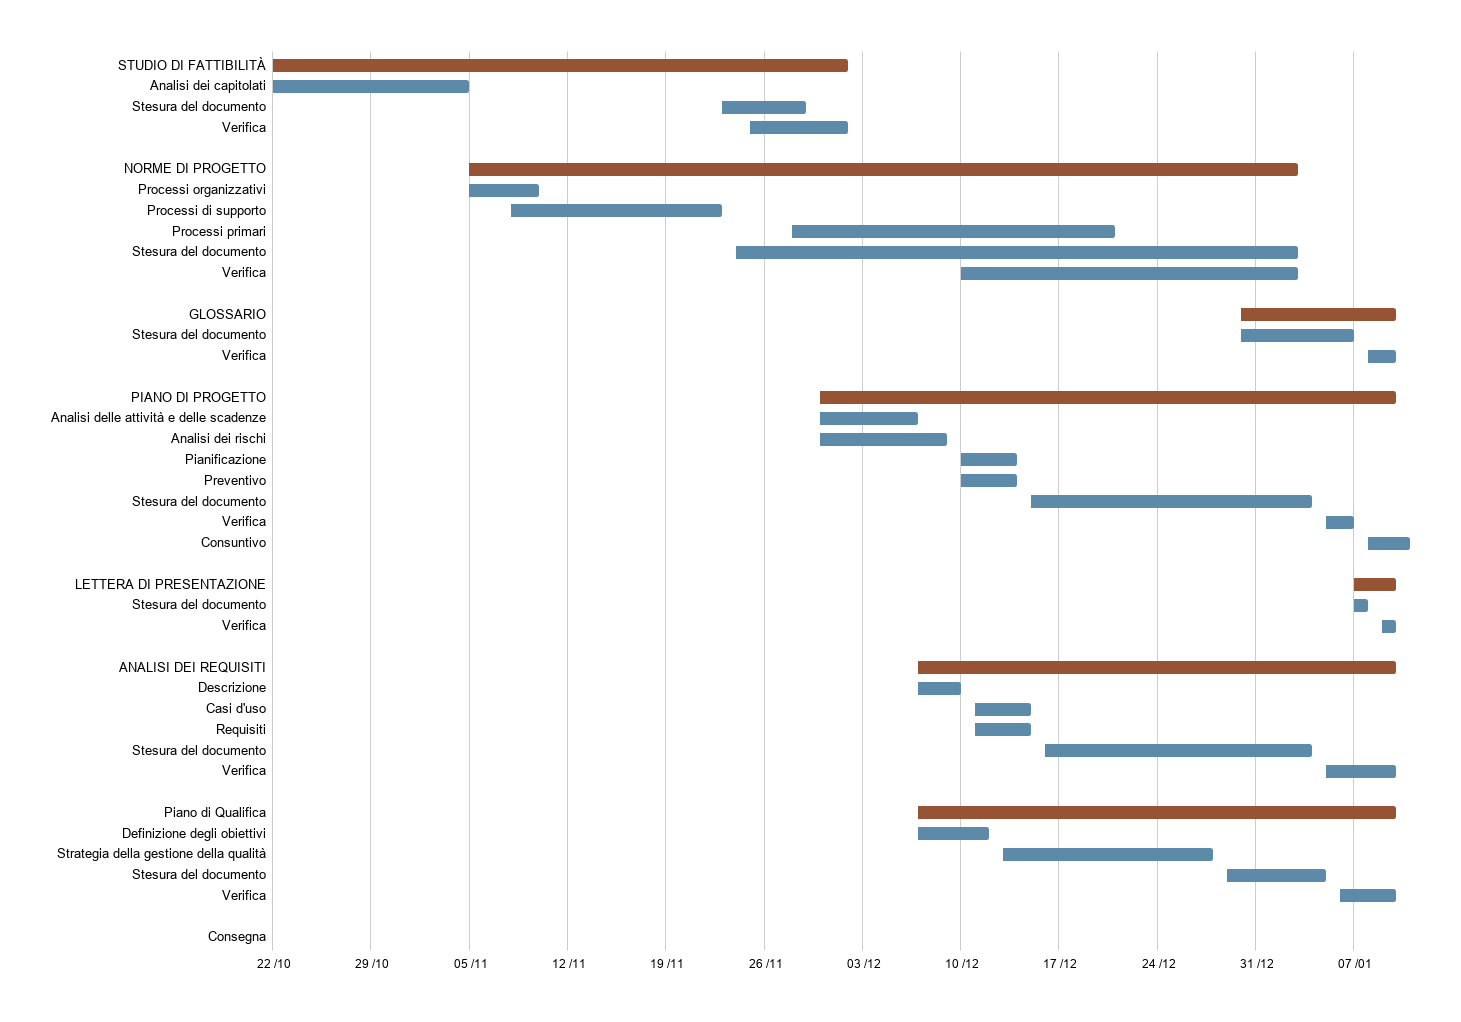
\includegraphics[width=1\linewidth]{../immagini/pdp/gantt_analisi.png}
		\caption{Diagramma di Gantt dell'attività di analisi}
	\end{center}
\end{figure}

\section{Consolidamento dei requisiti}\label{PianificazioneConsolidamentoDeiRequisiti}
\textbf{Periodo:} dal 11-01-2021 al 18-01-2021
Questo periodo ha inizio subito dopo il termine del precedente e finisce con la presentazione della Revisione dei Requisiti.
Il gruppo \textit{Jawa Druids} si dedicherà ai seguenti compiti$_{\scaleto{G}{3pt}}$:
\begin{itemize}
	\item avanzamento con lo studio individuale relativo a:
	\begin{itemize}
		\item acquisizione dei dati;
		\item simulazione dei dati;
		\item machine learning$_G$;
		\item web app.
	\end{itemize}
	\item preparazione del materiale necessario alla presentazione.
\end{itemize}
\subsection{Diagramma di Gantt: consolidamento dei requisiti}\label{PianificazioneDiagrammaDiGanttConsolidamento}
\begin{figure}[!h]
	\begin{center}
		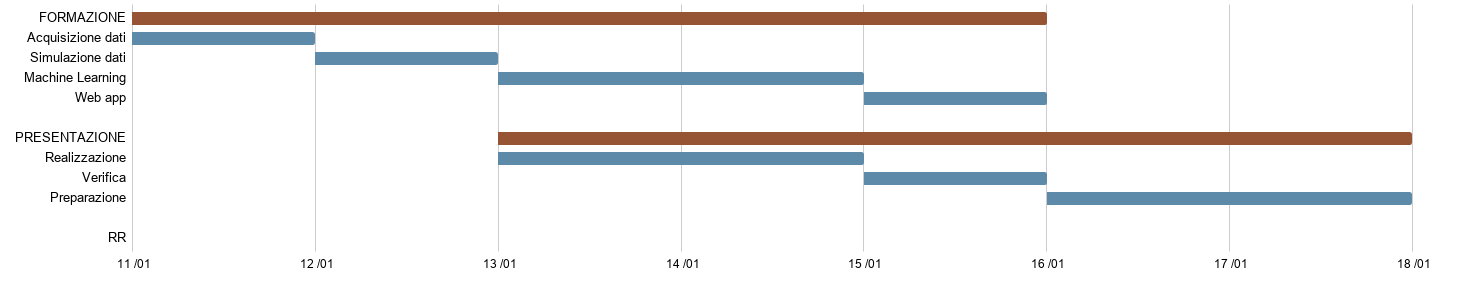
\includegraphics[width=1\linewidth]{../immagini/pdp/gantt_consolidamento_requisiti.png}
		\caption{Diagramma di Gantt del consolidamento dei requisiti}
	\end{center}
\end{figure}
\clearpage
\section{Progettazione architetturale}\label{PianificazioneProgettazioneArchitetturale}
\textbf{Periodo:} dal 19-01-2021 al 08-03-2021. \\
Questo periodo ha inizio subito dopo conclusione del precedente e termina con la Revisione di Progettazione.
Esso ha il compito di correggere ed incrementare la documentazione prodotta e di portare all'individuazione di una soluzione architetturale che permetta il soddisfacimento dei requisiti$_{\scaleto{G}{3pt}}$ obbligatori. È suddiviso in:
\begin{itemize}
	\item \textbf{Incremento e verifica:} analizzando l'esito della Revisione dei Requisiti, vengono svolte attività$_{\scaleto{G}{3pt}}$ di Incremento e Verifica sui vari documenti redatti, dove necessario;
	\item \textbf{Technology Baseline$_G$:} viene redatta la documentazione di supporto, contenente la descrizione delle tecnologie individuate e il tracciamento della relazione tra le componenti e i requisiti$_{\scaleto{G}{3pt}}$ che vanno a soddisfare.
	Viene realizzato un Proof of Concept$_G$ che verrà condiviso col proponente$_{\scaleto{G}{3pt}}$ per verificare il corretto sviluppo del software. In particolare il gruppo ha suddiviso ulteriormente questa fase in due incrementi:
	\begin{itemize}
		\item \textbf{Primo incremento -  15-02-2021 - 26-02-2021}: in questo periodo il gruppo svilupperà 5 moduli separati, ognuno riguardante un diverso aspetto del prodotto. In particolare i moduli 1 e 2 si occuperanno di ricavare il numero di persone presenti in un determinato luogo e istante di tempo partendo dal video di una webcam, produrranno in output un dato che conterrà tale informazione. Il modulo 3 dovrà prendere in input i dati che riceve dai moduli precedenti e salvarli nel database in modo da renderli disponibili per l'utilizzo. Il modulo 4 inizierà lo sviluppo di un modello di machine learning$_{\scaleto{G}{3pt}}$ in grado di fare previsioni future. Data la corposità di questo modulo, crediamo che questa funzionalità non sarà implementata nel Proof of Concept$_{\scaleto{G}{3pt}}$. Infine il quinto modulo si occuperà di prendere gli ultimi dati caricati nel database e visualizzarli in una heat map$_{\scaleto{G}{3pt}}$.
		\item \textbf{Secondo incremento - 27-02-2021 - 04-03-2021 }: nel periodo successivo il gruppo unirà tutti i prototipi dei moduli sviluppati in un unico Proof of Concept$_{\scaleto{G}{3pt}}$ che sia in grado di soddisfare alcuni dei casi d'uso$_{\scaleto{G}{3pt}}$ obbligatori. Tra questi il gruppo si pone come obiettivo che sia disponibile la heat map$_{\scaleto{G}{3pt}}$ (UC1) che prenda dati reali recentemente aggiunti al database (UC8.2), che vengano visualizzati i messaggi di errore in caso questi dati non siano disponibili (UC2 - UC9). Nel caso in cui ci sia la possibilità in termini di tempo, il Proof of Concept$_{\scaleto{G}{3pt}}$ continuerà ad essere sviluppato fino al termine della consegna, aggiungendo altri casi d'uso$_{\scaleto{G}{3pt}}$ obbligatori.
	\end{itemize}
\end{itemize}
\subsection{Primo Periodo}\label{PianificazioneProgettazioneArchitetturalePrimoPeriodo}
\textbf{19-01-2021 - 12-02-2021}: in questo primo periodo che, data la concomitanza con la sessione d'esami, risulta più esteso,  il gruppo inizierà la correzione dei documenti già redatti in concomitanza con la ricerca di fonti affidabili che ogni membro potrà consultare per fare formazione sulle tecnologie da utilizzare per la Technology Baseline$_{\scaleto{G}{3pt}}$.
\subsection{Secondo Periodo}\label{PianificazioneProgettazioneArchitetturaleSecondoPeriodo}
\textbf{13-02-2021 - 27-02-2021}: durante il secondo periodo il gruppo continuerà la propria formazione e deciderà come suddividere l'assegnazione dei moduli sopra citati. In seguito inizierà lo sviluppo degli stessi fino ad arrivare alla conclusione del primo incremento del Proof of Concept$_{\scaleto{G}{3pt}}$.
\subsection{Terzo Periodo}\label{PianificazioneProgettazioneArchitetturaleTerzoPeriodo}
\textbf{28-02-2021 - 08-03-2021}: in questo ultimo periodo il gruppo dovrà terminare anche il secondo incremento del Proof of Concept$_{\scaleto{G}{3pt}}$ ed ultimare la documentazione da presentare.

\subsection{Diagramma di Gantt: progettazione architetturale}\label{PianificazioneDiagrammaDiGanttProgettazioneArchitetturale}
\begin{figure}[h]
	\begin{center}
		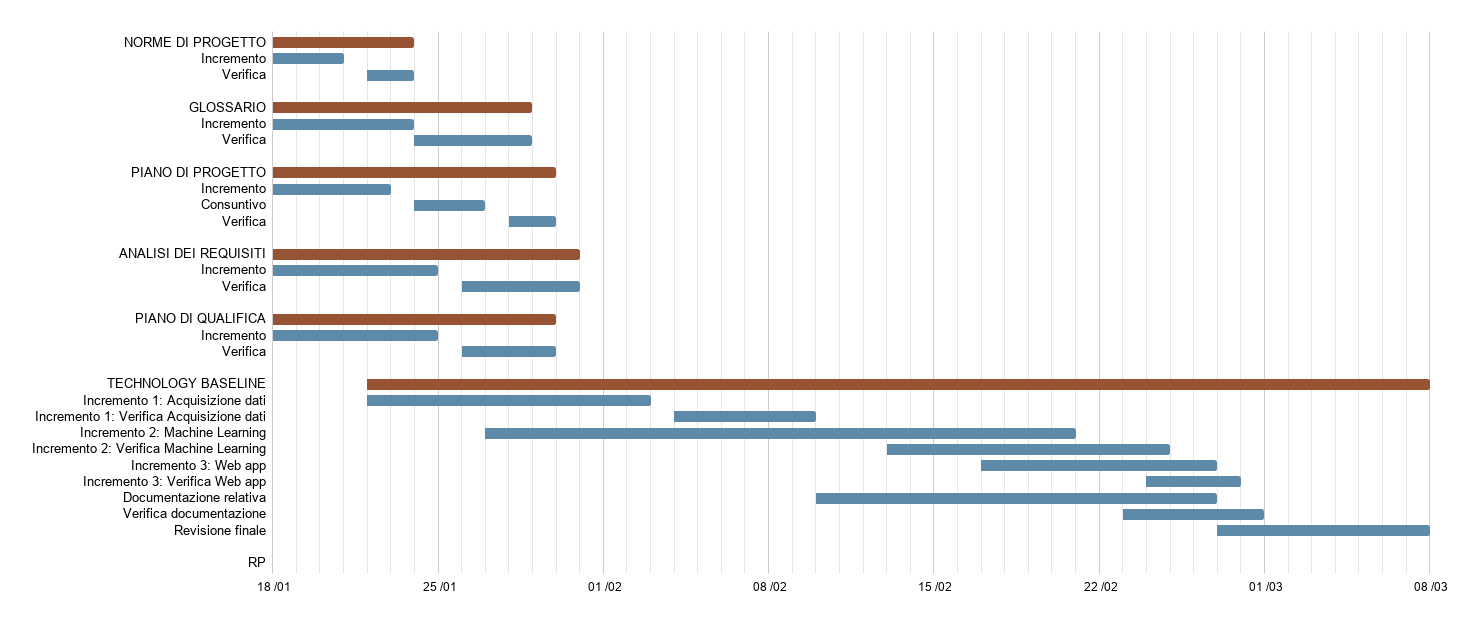
\includegraphics[width=0.9\linewidth]{../immagini/pdp/gantt_progettazione_architetturale.png}
		\caption{Diagramma di Gantt della progettazione architetturale}
	\end{center}
\end{figure}
\clearpage
\section{Progettazione di dettaglio e codifica}\label{PianificazioneProgettazioneDettaglio}
\textbf{Periodo:} dal 15-03-2021 al 09-04-2021
Questo periodo inizia appena concluso il precedente e termina con la Revisione di Qualifica.
Le principali attività$_{\scaleto{G}{3pt}}$ svolte in questo periodo sono
\begin{itemize}
	\item \textbf{Incremento e verifica:} alcuni dei documenti già prodotti vengono migliorati e aggiornati;
	\item \textbf{Product Baseline$_G$:} segue la Technology Baseline$_{\scaleto{G}{3pt}}$, dove vengono studiati meglio design pattern$_G$, classi e attività$_{\scaleto{G}{3pt}}$ necessarie alla codifica;
	\item \textbf{Specifica Tecnica:} è un documento contenente tutte le caratteristiche del prodotto e le motivazioni che hanno portato alla loro scelta;
	\item \textbf{Codifica:} attività$_{\scaleto{G}{3pt}}$ nella quale viene prodotto e verificato il codice;
	\item \textbf{Manuale utente:} attività$_{\scaleto{G}{3pt}}$ nella quale viene redatto il documento contenente le informazioni su come funziona e su come si utilizza il prodotto.
\end{itemize}
\subsection{Diagramma di Gantt: progettazione di dettaglio e codifica}\label{PianificazioneDiagrammaDiGanttProgettazioneDettaglio}
\begin{figure}[!h]
	\begin{center}
		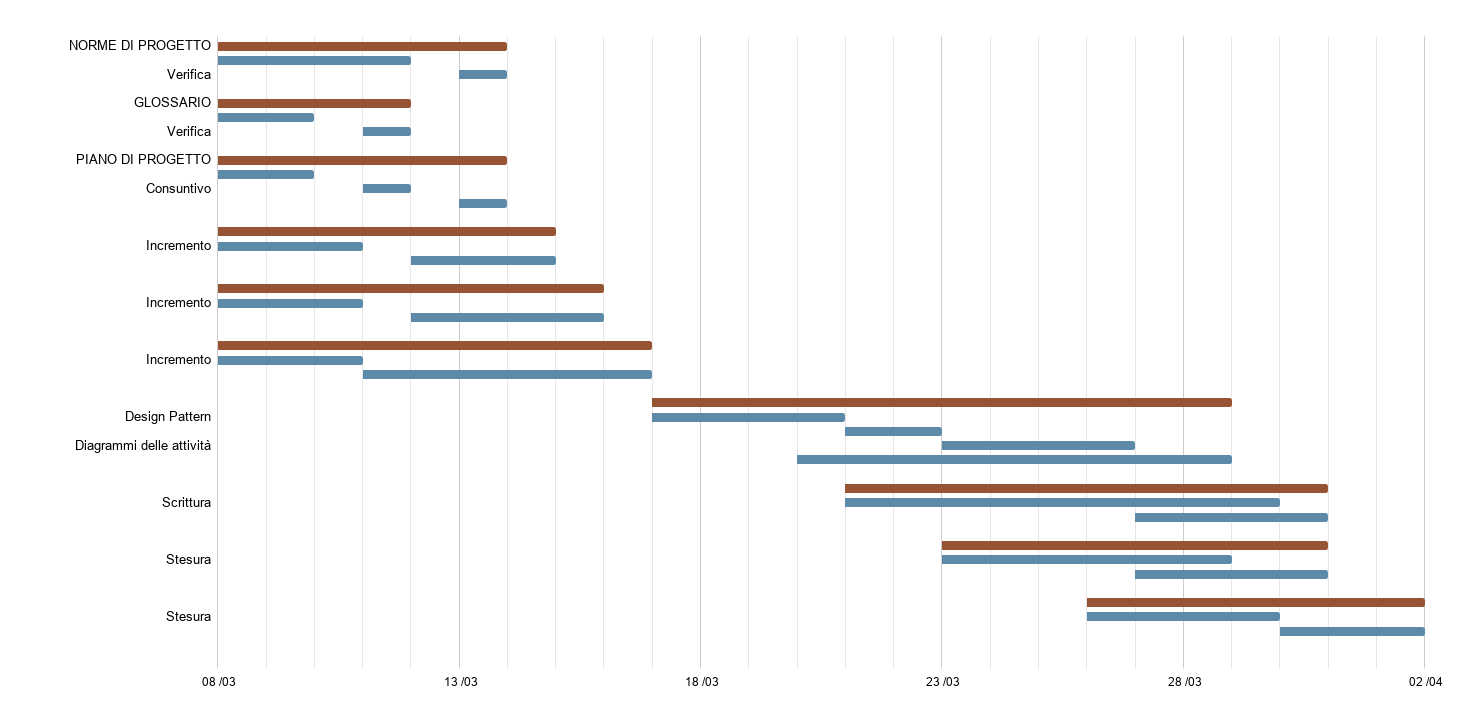
\includegraphics[width=0.8\linewidth]{../immagini/pdp/gantt_progettazione_dettaglio.png}
		\caption{Diagramma di Gantt dell'attività di progettazione di dettaglio e codifica}
	\end{center}
\end{figure}
\section{Validazione e Collaudo}\label{PianificazioneValidazione}
\textbf{Periodo:} dal 16-04-2021 al 10-05-2021
Questo periodo inizia appena concluso il precedente e termina con la Revisione di Accettazione.
Le principali attività$_{\scaleto{G}{3pt}}$ svolte in questo periodo sono:
\begin{itemize}
	\item \textbf{Incremento e verifica:} analizzando l'esito della Revisione di Qualifica vengono svolte attività$_{\scaleto{G}{3pt}}$ di Incremento e Verifica sui vari documenti redatti;
	\item \textbf{Validazione e Collaudo:} vengono realizzati gli ultimi test, con i dovuti controlli finali, in modo da garantire un buon livello di qualità e correttezza.
\end{itemize}
\subsection{Diagramma di Gantt: validazione e collaudo}\label{PianificazioneDiagrammaDiGanttValidazione}
\begin{figure}[!h]
	\begin{center}
		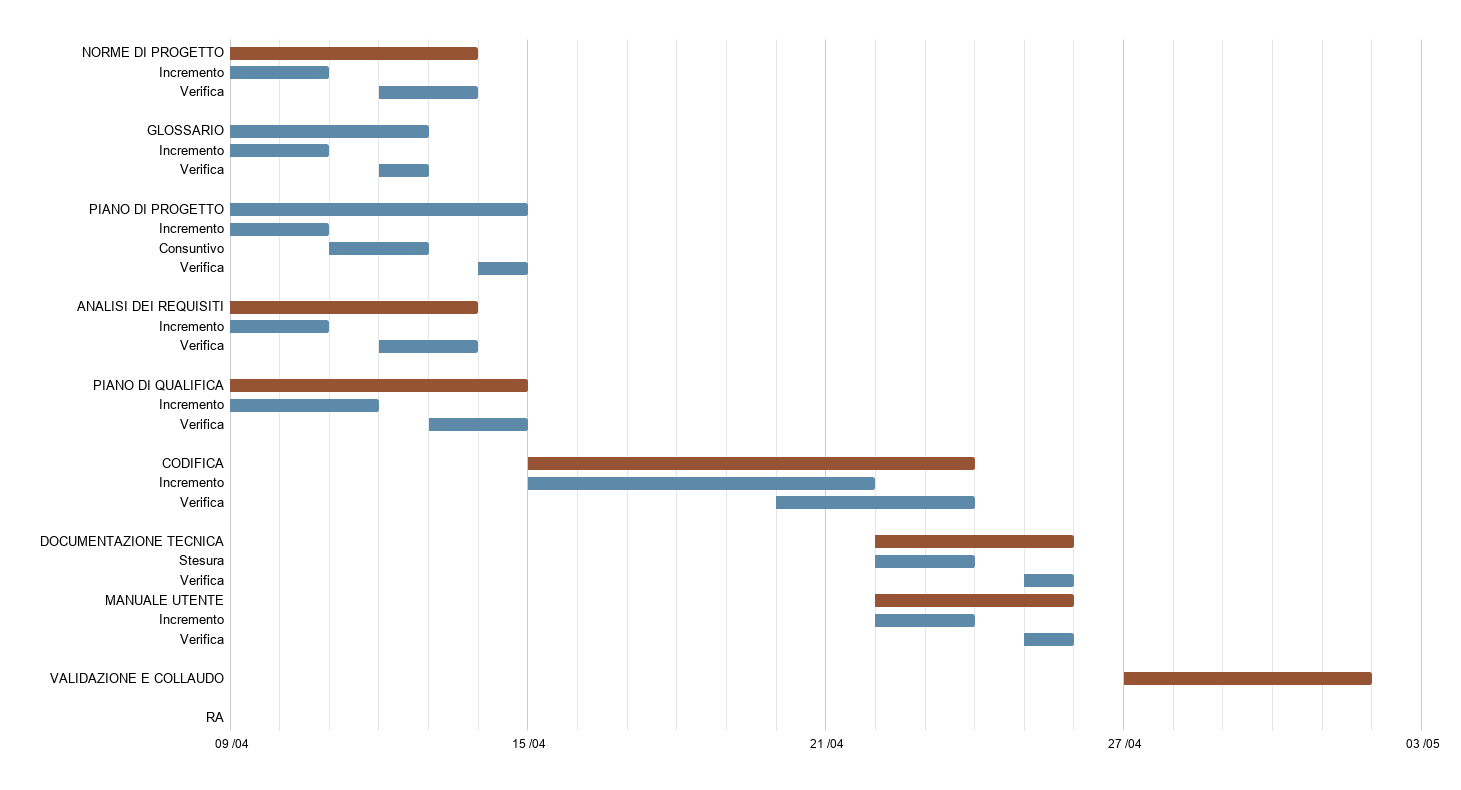
\includegraphics[width=0.8\linewidth]{../immagini/pdp/gantt_validazione.png}
		\caption{Diagramma di Gantt dell'attività di validazione e collaudo}
	\end{center}
\end{figure}

\chapter{Preventivo}\label{Preventivo}

In questa sezione il gruppo \textit{Jawa Druids} descrive come userà le risorse a sua disposizione. Per identificarli nelle tabelle, i ruoli vengono indicati con le seguenti sigle:
\begin{itemize}
	\item \textbf{Re}: \textit{Responsabile};
	\item \textbf{Am}: \textit{Amministratore};
	\item \textbf{An}: \textit{Analista};
	\item \textbf{Pt}: \textit{Progettista};
	\item \textbf{Pr}: \textit{Programmatore};
	\item \textbf{Ve}: \textit{Verificatore}.
\end{itemize}
\clearpage
\section{Fase di Analisi}\label{PreventivoFaseDiAnalisi}

\subsection{Prospetto orario}\label{PreventivoFaseDiAnalisiProspettoOrario}
In questa fase la distribuzione oraria è la seguente:
\quad
\def\tabularxcolumn#1{m{#1}}
{\rowcolors{2}{RawSienna!90!RawSienna!20}{RawSienna!70!RawSienna!40}

	\begin{center}
		\renewcommand{\arraystretch}{1.4}
		\begin{tabularx}{\textwidth}{|X|c|c|c|c|c|c|c|}
			\hline
			\rowcolor{airforceblue}
			\textbf{Nominativo} & \textbf{Re} & \textbf{Am} & \textbf{An} & \textbf{Pt} & \textbf{Pr} & \textbf{Ve} & \textbf{Totale ore}\\
			\hline
			\textit{Andrea Dorigo} & 10 & 7 & 3 & 0 & 0 & 5 & 25\\
			\hline
			\textit{Margherita Mitillo} & 8 & 3 & 13 & 0 & 0 & 1 & 25\\
			\hline
			\textit{Igli Mezini} & 3 & 6 & 8 & 0 & 0 & 8 & 25\\
			\hline
			\textit{Andrea Cecchin} & 5 & 9 & 9 & 0 & 0 & 2 & 25\\
			\hline
			\textit{Emma Roveroni} & 2 & 5 & 7 & 0 & 0 & 11 & 25\\
			\hline
			\textit{Alfredo Graziano} & 0 & 10 & 9 & 0 & 0 & 6 & 25\\
			\hline
			\textit{Mattia Cocco} & 1 & 9 & 8 & 0 & 0 & 7 & 25\\
			\hline
			Totale ore ruolo & 29 & 49 & 57 & 0 & 0 & 40 & 175\\
			\hline
		\end{tabularx}
	\captionof{table}{\textbf{Distribuzione delle ore durante l'Analisi}}
	\end{center}

Il seguente istogramma riassume i dati ottenuti:
\begin{figure}[!h]
	\begin{center}
		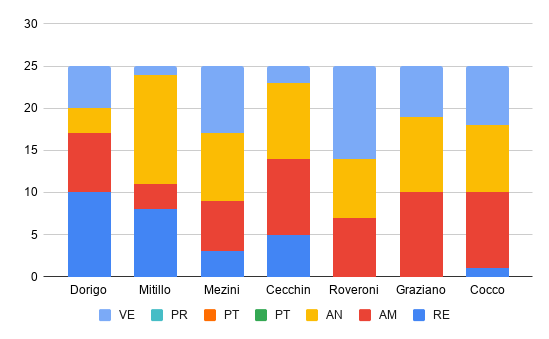
\includegraphics[width=0.7\linewidth]{../immagini/pdp/istogramma_analisi.png}
		\caption{Istogramma della ripartizione oraria durante la Analisi}
	\end{center}
\end{figure}
\clearpage
\subsection{Prospetto economico}\label{PreventivoFaseDiAnalisiProspettoEconomico}
\quad
\def\tabularxcolumn#1{m{#1}}
{\rowcolors{2}{RawSienna!90!RawSienna!20}{RawSienna!70!RawSienna!40}
	\begin{center}
		\renewcommand{\arraystretch}{1.4}
		\begin{tabularx}{7cm}{|X|c|c|}
			\hline
			\rowcolor{airforceblue}
			\textbf{Ruolo} & \textbf{Ore} & \textbf{Costo}\\
			\hline
			Responsabile & 29 & 870\euro\\
			\hline
			Amministratore & 49 & 980\euro\\
			\hline
			Analista & 57 & 1425\euro\\
			\hline
			Progettista & 0 & 0\euro\\
			\hline
			Programmatore & 0 & 0\euro\\
			\hline
			Verificatore & 40 & 600\euro\\
			\hline
			Totale & 175 & 3875\euro\\
			\hline
		\end{tabularx}
	\captionof{table}{\textbf{Prospetto dei costi per ruolo nel periodo di Analisi}}
	\end{center}
Il seguente grafico a torta riassume i dati ottenuti:
\begin{figure}[!ht]
	\begin{center}
		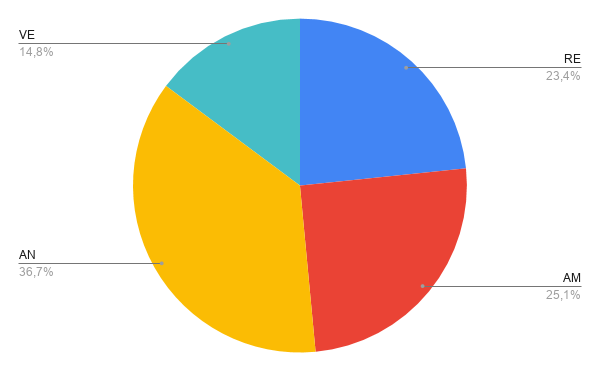
\includegraphics[width=0.8\linewidth]{../immagini/pdp/torta_analisi.png}
		\caption{Grafico a torta della ripartizione per ruolo delle ore nel periodo di Analisi}
	\end{center}
\end{figure}
\clearpage
\section{Fase di Consolidamento dei requisiti}\label{PreventivoFaseDiConsolidamentoDeiRequisiti}

\subsection{Prospetto orario}\label{PreventivoFaseDiConsolidamentoDeiRequisitiProspettoOrario}
In questa fase la distribuzione oraria è la seguente:
\quad
\def\tabularxcolumn#1{m{#1}}
{\rowcolors{2}{RawSienna!90!RawSienna!20}{RawSienna!70!RawSienna!40}

	\begin{center}
		\renewcommand{\arraystretch}{1.4}
		\begin{tabularx}{\textwidth}{|X|c|c|c|c|c|c|c|}
			\hline
			\rowcolor{airforceblue}
			\textbf{Nominativo} & \textbf{Re} & \textbf{Am} & \textbf{An} & \textbf{Pt} & \textbf{Pr} & \textbf{Ve} & \textbf{Totale ore}\\
			\hline
			\textit{Andrea Dorigo} & 0 & 2 & 0 & 0 & 0 & 2 & 4\\
			\hline
			\textit{Margherita Mitillo} & 0 & 2 & 1 & 0 & 0 & 1 & 4\\
			\hline
			\textit{Igli Mezini} & 1 & 1 & 0 & 0 & 0 & 2 & 4\\
			\hline
			\textit{Andrea Cecchin} & 1 & 0 & 2 & 0 & 0 & 1 & 4\\
			\hline
			\textit{Emma Roveroni} & 1 & 1 & 0 & 0 & 0 & 2 & 4\\
			\hline
			\textit{Alfredo Graziano} & 1 & 2 & 1 & 0 & 0 & 0 & 4\\
			\hline
			\textit{Mattia Cocco} & 1 & 0 & 1 & 0 & 0 & 2 & 4\\
			\hline
			Totale ore ruolo & 5 & 8 & 5 & 0 & 0 & 10 & 28\\
			\hline
		\end{tabularx}
	\captionof{table}{\textbf{Distribuzione delle ore durante il Consolidamento dei requisiti}}
	\end{center}
Il seguente istogramma riassume i dati ottenuti:
\begin{figure}[!ht]
	\begin{center}
		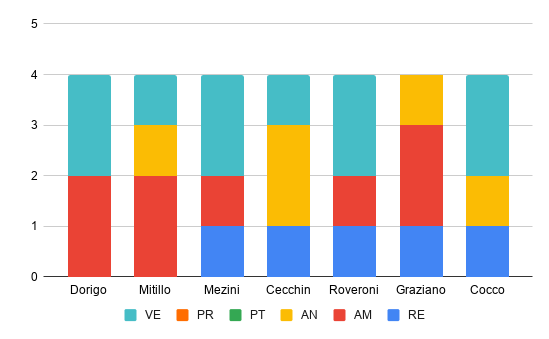
\includegraphics[width=0.7\linewidth]{../immagini/pdp/istogramma_consolidamento_requisiti.png}
		\caption{Istogramma della ripartizione oraria durante il Consolidamento dei requisiti
}
	\end{center}
\end{figure}

\subsection{Prospetto economico}\label{PreventivoFaseDiConsolidamentoDeiRequisitiProspettoEconomico}
\quad
\def\tabularxcolumn#1{m{#1}}
{\rowcolors{2}{RawSienna!90!RawSienna!20}{RawSienna!70!RawSienna!40}
	\begin{center}
		\renewcommand{\arraystretch}{1.4}
		\begin{tabularx}{7cm}{|X|c|c|}
			\hline
			\rowcolor{airforceblue}
			\textbf{Ruolo} & \textbf{Ore} & \textbf{Costo}\\
			\hline
			Responsabile & 5 & 150\euro\\
			\hline
			Amministratore & 8 & 160\euro\\
			\hline
			Analista & 5 & 125\euro\\
			\hline
			Progettista & 0 & 0\euro\\
			\hline
			Programmatore & 0 & 0\euro\\
			\hline
			Verificatore & 10 & 150\euro\\
			\hline
			Totale & 28 & 585\euro\\
			\hline
		\end{tabularx}
	\captionof{table}{\textbf{Prospetto dei costi per ruolo nel periodo di Consolidamento dei requisiti}}
	\end{center}
Il seguente grafico a torta riassume i dati ottenuti:
\begin{figure}[!ht]
	\begin{center}
		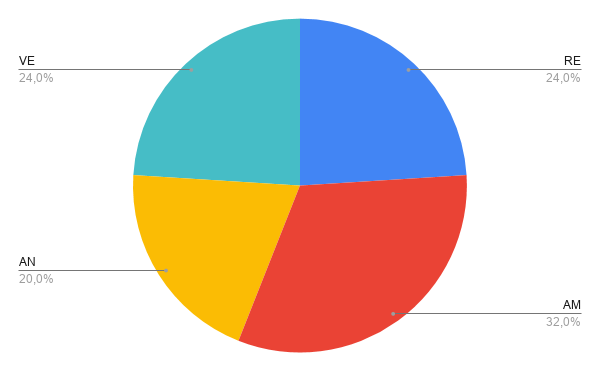
\includegraphics[width=0.8\linewidth]{../immagini/pdp/torta_consolidamento_requisiti.png}
		\caption{Grafico a torta della ripartizione per ruolo delle ore durante il periodo di Consolidamento dei requisiti}
	\end{center}
\end{figure}

\section{Fase di Progettazione architetturale}\label{PreventivoFaseDiProgettazioneArchitetturale}

\subsection{Prospetto orario}\label{PreventivoFaseDiProgettazioneArchitetturaleProspettoOrario}
In questa fase la distribuzione oraria è la seguente:
\quad
\def\tabularxcolumn#1{m{#1}}
{\rowcolors{2}{RawSienna!90!RawSienna!20}{RawSienna!70!RawSienna!40}

	\begin{center}
		\renewcommand{\arraystretch}{1.4}
		\begin{tabularx}{\textwidth}{|X|c|c|c|c|c|c|c|}
			\hline
			\rowcolor{airforceblue}
			\textbf{Nominativo} & \textbf{Re} & \textbf{Am} & \textbf{An} & \textbf{Pt} & \textbf{Pr} & \textbf{Ve} & \textbf{Totale ore}\\
			\hline
			\textit{Andrea Dorigo} & 5 & 3 & 2 & 16 & 4 & 5 & 35\\
			\hline
			\textit{Margherita Mitillo} & 5 & 7 & 2 & 12 & 0 & 9 & 35\\
			\hline
			\textit{Igli Mezini} & 4 & 2 & 8 & 8 & 3 & 10 & 35\\
			\hline
			\textit{Andrea Cecchin} & 7 & 5 & 4 & 10 & 2 & 7 & 35\\
			\hline
			\textit{Emma Roveroni} & 1 & 7 & 4 & 14 & 0 & 9 & 35\\
			\hline
			\textit{Alfredo Graziano} & 2 & 2 & 9 & 15 & 2 & 5 & 35\\
			\hline
			\textit{Mattia Cocco} & 6 & 2 & 6 & 11 & 1 & 9 & 35\\
			\hline
			Totale ore ruolo & 30 & 28 & 35 & 86 & 12 & 54 & 245\\
			\hline
		\end{tabularx}
	\captionof{table}{\textbf{distribuzione delle ore durante la Progettazione architetturale}}
	\end{center}

Il seguente istogramma riassume i dati ottenuti:
\begin{figure}[!h]
	\begin{center}
		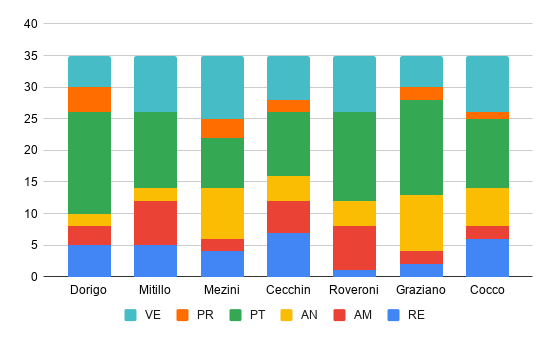
\includegraphics[width=0.7\linewidth]{../immagini/pdp/istogramma_progettazione_architetturale.png}
		\caption{Istogramma della ripartizione oraria durante la Progettazione architetturale}
	\end{center}
\end{figure}

\subsection{Prospetto economico}\label{PreventivoFaseDiProgettazioneArchitetturaleProspettoEconomico}
\quad
\def\tabularxcolumn#1{m{#1}}
{\rowcolors{2}{RawSienna!90!RawSienna!20}{RawSienna!70!RawSienna!40}
	\begin{center}
		\renewcommand{\arraystretch}{1.4}
		\begin{tabularx}{7cm}{|X|c|c|}
			\hline
			\rowcolor{airforceblue}
			\textbf{Ruolo} & \textbf{Ore} & \textbf{Costo}\\
			\hline
			Responsabile & 30 & 900\euro\\
			\hline
			Amministratore & 28 & 560\euro\\
			\hline
			Analista & 35 & 875\euro\\
			\hline
			Progettista & 86 & 1892\euro\\
			\hline
			Programmatore & 12 & 180\euro\\
			\hline
			Verificatore & 54 & 810\euro\\
			\hline
			Totale & 245 & 5217\euro\\
			\hline
		\end{tabularx}
	\captionof{table}{\textbf{Prospetto dei costi per ruolo nel periodo di Progettazione architetturale}}
	\end{center}

Il seguente grafico a torta riassume i dati ottenuti:
\begin{figure}[!ht]
	\begin{center}
		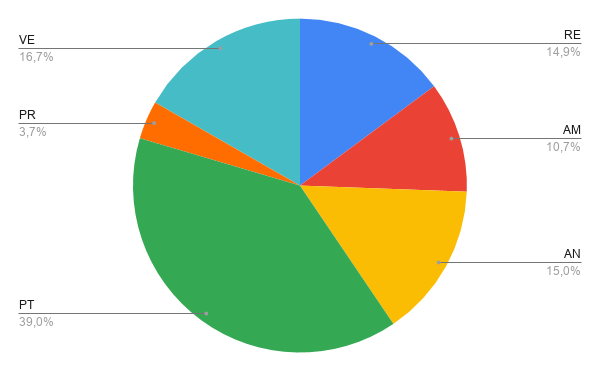
\includegraphics[width=0.8\linewidth]{../immagini/pdp/torta_progettazione_architetturale.png}
		\caption{Grafico a torta della ripartizione per ruolo delle ore nel periodo di Progettazione architetturale}
	\end{center}
\end{figure}

\section{Fase di Progettazione di dettaglio e codifica}\label{PreventivoFaseDiProgettazioneDiDettaglioECodifica}

\subsection{Primo Periodo}\label{PreventivoFaseDiProgettazioneDiDettaglioECodificaPeriodo1}

\subsubsection{Prospetto delle ore degli incrementi}\label{PreventivoFaseDiProgettazioneDiDettaglioECodificaPeriodo1Incrementi}
Di seguito riportiamo la previsione delle ore che ciascun incremento necessita, relativamente a questo periodo.
\quad
\def\tabularxcolumn#1{m{#1}}
{\rowcolors{2}{RawSienna!90!RawSienna!20}{RawSienna!70!RawSienna!40}

	\begin{center}
		\renewcommand{\arraystretch}{1.4}
		\begin{tabularx}{\textwidth}{|X|c|c|c|c|c|c|c|}
			\hline
			\rowcolor{airforceblue}
			\textbf{Incremento} & \textbf{Re} & \textbf{Am} & \textbf{An} & \textbf{Pt} & \textbf{Pr} & \textbf{Ve} & \textbf{Totale ore}\\
			\hline
			\textit{Incremento 1} & 5 & 3 & 19 & 5 & 0 & 14 & 46\\
			\hline
			\textit{Incremento 2} & 3 & 0 & 0 & 15 & 20 & 0 & 38\\
			\hline
			Totale ore ruolo & 8 & 3 & 19 & 20 & 20 & 14 & 84\\
			\hline
		\end{tabularx}
		\captionof{table}{\textbf{Prospetto delle ore degli incrementi del primo periodo della fase di Progettazione di dettaglio e codifica}}
	\end{center}

\subsubsection{Prospetto orario}\label{PreventivoFaseDiProgettazioneDiDettaglioECodificaProspettoOrarioPeriodo1}
In questa fase la distribuzione oraria è la seguente:
\quad
\def\tabularxcolumn#1{m{#1}}
{\rowcolors{2}{RawSienna!90!RawSienna!20}{RawSienna!70!RawSienna!40}

	\begin{center}
		\renewcommand{\arraystretch}{1.4}
		\begin{tabularx}{\textwidth}{|X|c|c|c|c|c|c|c|}
			\hline
			\rowcolor{airforceblue}
			\textbf{Nominativo} & \textbf{Re} & \textbf{Am} & \textbf{An} & \textbf{Pt} & \textbf{Pr} & \textbf{Ve} & \textbf{Totale ore}\\
			\hline
			\textit{Andrea Dorigo} & 3 & 0 & 3 & 4 & 2 & 1 & 13\\
			\hline
			\textit{Margherita Mitillo} & 0 & 0 & 4 & 3 & 2 & 2 & 11\\
			\hline
			\textit{Igli Mezini} & 2 & 0 & 6 & 1 & 0 & 2 & 11\\
			\hline
			\textit{Andrea Cecchin} & 0 & 3 & 0 & 4 & 5 & 2 & 14\\
			\hline
			\textit{Emma Roveroni} & 0 & 0 & 0 & 3 & 6 & 2 & 11\\
			\hline
			\textit{Alfredo Graziano} & 3 & 0 & 6 & 0 & 0 & 3 & 12\\
			\hline
			\textit{Mattia Cocco} & 0 & 0 & 0 & 5 & 5 & 2 & 12\\
			\hline
			Totale ore ruolo & 8 & 3 & 19 & 20 & 20 & 14 & 84\\
			\hline
		\end{tabularx}
	\captionof{table}{\textbf{Distribuzione delle ore del primo periodo della fase di Progettazione di dettaglio e codifica}}
	\end{center}
Il seguente istogramma riassume i dati ottenuti:
\begin{figure}[!h]
	\begin{center}
		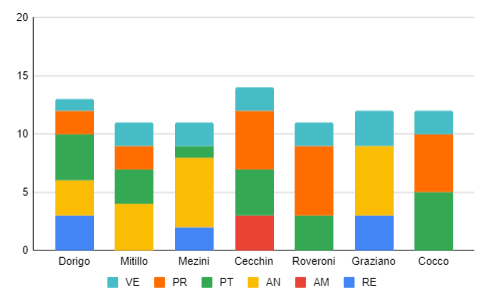
\includegraphics[width=0.7\linewidth]{../immagini/pdp/istogramma_progettazione_dettaglio_periodo1.png}
		\caption{Istogramma della ripartizione oraria durante il primo periodo della fase di Progettazione di
			dettaglio e codifica}
	\end{center}
\end{figure}
\clearpage
\subsubsection{Prospetto economico}\label{PreventivoFaseDiProgettazioneDiDettaglioECodificaProspettoEconomicoPeriodo1}
\quad
\def\tabularxcolumn#1{m{#1}}
{\rowcolors{2}{RawSienna!90!RawSienna!20}{RawSienna!70!RawSienna!40}
	\begin{center}
		\renewcommand{\arraystretch}{1.4}
		\begin{tabularx}{7cm}{|X|c|c|}
			\hline
			\rowcolor{airforceblue}
			\textbf{Ruolo} & \textbf{Ore} & \textbf{Costo}\\
			\hline
			Responsabile & 8 & 240\euro\\
			\hline
			Amministratore & 3 & 60\euro\\
			\hline
			Analista & 19 & 475\euro\\
			\hline
			Progettista & 20 & 440\euro\\
			\hline
			Programmatore & 20 & 300\euro\\
			\hline
			Verificatore & 14 & 210\euro\\
			\hline
			Totale & 84 & 1725\euro\\
			\hline
		\end{tabularx}
	\captionof{table}{\textbf{Prospetto dei costi per ruolo nel primo periodo della fase di Progettazione di dettaglio e codifica}}
	\end{center}

Il seguente grafico a torta riassume i dati ottenuti:
\begin{figure}[!ht]
	\begin{center}
		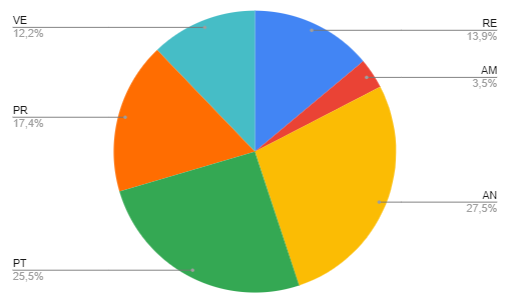
\includegraphics[width=0.8\linewidth]{../immagini/pdp/torta_progettazione_dettaglio_periodo1.png}
		\caption{Grafico a torta della ripartizione dei costi per ruolo del primo periodo della fase di Progettazione e codifica}
	\end{center}
\end{figure}

\subsection{Secondo Periodo}\label{PreventivoFaseDiProgettazioneDiDettaglioECodificaPeriodo2}

\subsubsection{Prospetto delle ore degli incrementi}\label{PreventivoFaseDiProgettazioneDiDettaglioECodificaPeriodo2Incrementi}
Di seguito riportiamo la previsione delle ore che ciascun incremento necessita, relativamente a questo periodo.
\quad
\def\tabularxcolumn#1{m{#1}}
{\rowcolors{2}{RawSienna!90!RawSienna!20}{RawSienna!70!RawSienna!40}

	\begin{center}
		\renewcommand{\arraystretch}{1.4}
		\begin{tabularx}{\textwidth}{|X|c|c|c|c|c|c|c|}
			\hline
			\rowcolor{airforceblue}
			\textbf{Incremento} & \textbf{Re} & \textbf{Am} & \textbf{An} & \textbf{Pt} & \textbf{Pr} & \textbf{Ve} & \textbf{Totale ore}\\
			\hline
			\textit{Incremento 3} & 2 & 3 & 0 & 7 & 13 & 0 & 25\\
			\hline
			\textit{Incremento 4} & 5 & 6 & 7 & 0 & 0 & 16 & 34\\
			\hline
			\textit{Incremento 5} & 2 & 4 & 0 & 11 & 18 & 0 & 35\\
			\hline
			\textit{Incremento 6} & 1 & 2 & 0 & 2 & 4 & 0 & 9\\
			\hline
			\textit{Incremento 7} & 1 & 2 & 0 & 1 & 3 & 0 & 7\\
			\hline
			\textit{Incremento 8} & 5 & 6 & 0 & 5 & 13 & 0 & 29\\
			\hline
			\textit{Incremento 9} & 6 & 7 & 0 & 13 & 0 & 16 & 42\\
			\hline
			Totale ore ruolo & 22 & 30 & 7 & 39 & 51 & 32 & 181\\
			\hline
		\end{tabularx}
		\captionof{table}{\textbf{Prospetto delle ore degli incrementi del secondo periodo della fase di Progettazione di dettaglio e codifica}}
	\end{center}

	\subsubsection{Prospetto orario}\label{PreventivoFaseDiProgettazioneDiDettaglioECodificaProspettoOrarioPeriodo2}
	In questa fase la distribuzione oraria è la seguente:
	\quad
	\def\tabularxcolumn#1{m{#1}}
	{\rowcolors{2}{RawSienna!90!RawSienna!20}{RawSienna!70!RawSienna!40}

		\begin{center}
			\renewcommand{\arraystretch}{1.4}
			\begin{tabularx}{\textwidth}{|X|c|c|c|c|c|c|c|}
				\hline
				\rowcolor{airforceblue}
				\textbf{Nominativo} & \textbf{Re} & \textbf{Am} & \textbf{An} & \textbf{Pt} & \textbf{Pr} & \textbf{Ve} & \textbf{Totale ore}\\
				\hline
				\textit{Andrea Dorigo} & 6 & 4 & 0 & 3 & 8 & 4 & 25\\
				\hline
				\textit{Margherita Mitillo} & 3 & 3 & 3 & 3 & 10 & 6 & 28\\
				\hline
				\textit{Igli Mezini} & 5 & 5 & 0 & 10 & 0 & 7 & 27\\
				\hline
				\textit{Andrea Cecchin} & 0 & 5 & 0 & 5 & 13 & 0 & 23\\
				\hline
				\textit{Emma Roveroni} & 3 & 4 & 2 & 5 & 8 & 4 & 26\\
				\hline
				\textit{Alfredo Graziano} & 5 & 6 & 0 & 8 & 0 & 7 & 26\\
				\hline
				\textit{Mattia Cocco} & 0 & 3 & 2 & 5 & 12 & 4 & 26\\
				\hline
				Totale ore ruolo & 22 & 30 & 7 & 39 & 51 & 32 & 181\\
				\hline
			\end{tabularx}
			\captionof{table}{\textbf{Distribuzione delle ore del secondo periodo della fase di Progettazione di dettaglio e codifica}}
		\end{center}
		Il seguente istogramma riassume i dati ottenuti:
		\begin{figure}[!h]
			\begin{center}
				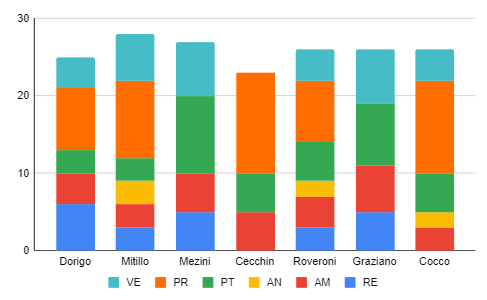
\includegraphics[width=0.7\linewidth]{../immagini/pdp/istogramma_progettazione_dettaglio_periodo2.png}
				\caption{Istogramma della ripartizione oraria durante il secondo periodo della fase di Progettazione di
					dettaglio e codifica}
			\end{center}
		\end{figure}
		\clearpage
		\subsubsection{Prospetto economico}\label{PreventivoFaseDiProgettazioneDiDettaglioECodificaProspettoEconomicoPeriodo2}
		\quad
		\def\tabularxcolumn#1{m{#1}}
		{\rowcolors{2}{RawSienna!90!RawSienna!20}{RawSienna!70!RawSienna!40}
			\begin{center}
				\renewcommand{\arraystretch}{1.4}
				\begin{tabularx}{7cm}{|X|c|c|}
					\hline
					\rowcolor{airforceblue}
					\textbf{Ruolo} & \textbf{Ore} & \textbf{Costo}\\
					\hline
					Responsabile & 22 & 660\euro\\
					\hline
					Amministratore & 30 & 600\euro\\
					\hline
					Analista & 7 & 175\euro\\
					\hline
					Progettista & 39 & 858\euro\\
					\hline
					Programmatore & 51 & 765\euro\\
					\hline
					Verificatore & 32 & 480\euro\\
					\hline
					Totale & 181 & 3538\euro\\
					\hline
				\end{tabularx}
				\captionof{table}{\textbf{Prospetto dei costi per ruolo nel secondo periodo della fase di Progettazione di dettaglio e codifica}}
			\end{center}

			Il seguente grafico a torta riassume i dati ottenuti:
			\begin{figure}[!ht]
				\begin{center}
					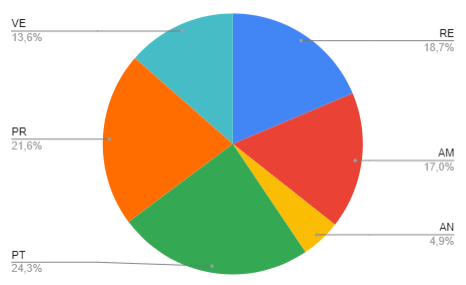
\includegraphics[width=0.8\linewidth]{../immagini/pdp/torta_progettazione_dettaglio_periodo2.png}
					\caption{Grafico a torta della ripartizione dei costi per ruolo del secondo periodo della fase di Progettazione e codifica}
				\end{center}
			\end{figure}

\subsection{Terzo Periodo}\label{PreventivoFaseDiProgettazioneDiDettaglioECodificaPeriodo3}

\subsubsection{Prospetto delle ore degli incrementi}\label{PreventivoFaseDiProgettazioneDiDettaglioECodificaPeriodo3Incrementi}
Di seguito riportiamo la previsione delle ore che ciascun incremento necessita, relativamente a questo periodo.
\quad
\def\tabularxcolumn#1{m{#1}}
{\rowcolors{2}{RawSienna!90!RawSienna!20}{RawSienna!70!RawSienna!40}

	\begin{center}
		\renewcommand{\arraystretch}{1.4}
		\begin{tabularx}{\textwidth}{|X|c|c|c|c|c|c|c|}
			\hline
			\rowcolor{airforceblue}
			\textbf{Incremento} & \textbf{Re} & \textbf{Am} & \textbf{An} & \textbf{Pt} & \textbf{Pr} & \textbf{Ve} & \textbf{Totale ore}\\
			\hline
			\textit{Incremento 10} & 3 & 3 & 0 & 8 & 0 & 30 & 44\\
			\hline
			\textit{Incremento 11} & 2 & 2 & 0 & 2 & 0 & 0 & 6\\
			\hline
			Totale ore ruolo & 5 & 5 & 0 & 10 & 0 & 30 & 50\\
			\hline
		\end{tabularx}
		\captionof{table}{\textbf{Prospetto delle ore degli incrementi del terzo periodo della fase di Progettazione di dettaglio e codifica}}
	\end{center}

	\subsubsection{Prospetto orario}\label{PreventivoFaseDiProgettazioneDiDettaglioECodificaProspettoOrarioPeriodo3}
	In questa fase la distribuzione oraria è la seguente:
	\quad
	\def\tabularxcolumn#1{m{#1}}
	{\rowcolors{2}{RawSienna!90!RawSienna!20}{RawSienna!70!RawSienna!40}

		\begin{center}
			\renewcommand{\arraystretch}{1.4}
			\begin{tabularx}{\textwidth}{|X|c|c|c|c|c|c|c|}
				\hline
				\rowcolor{airforceblue}
				\textbf{Nominativo} & \textbf{Re} & \textbf{Am} & \textbf{An} & \textbf{Pt} & \textbf{Pr} & \textbf{Ve} & \textbf{Totale ore}\\
				\hline
				\textit{Andrea Dorigo} & 2 & 0 & 0 & 0 & 0 & 5 & 7\\
				\hline
				\textit{Margherita Mitillo} & 0 & 1 & 0 & 2 & 0 & 3 & 6\\
				\hline
				\textit{Igli Mezini} & 2 & 0 & 0 & 3 & 0 & 2 & 7\\
				\hline
				\textit{Andrea Cecchin} & 0 & 2 & 0 & 0 & 0 & 6 & 8\\
				\hline
				\textit{Emma Roveroni} & 0 & 1 & 0 & 2 & 0 & 5 & 8\\
				\hline
				\textit{Alfredo Graziano} & 1 & 0 & 0 & 3 & 0 & 3 & 7\\
				\hline
				\textit{Mattia Cocco} & 0 & 1 & 0 & 0 & 0 & 6 & 7\\
				\hline
				Totale ore ruolo & 5 & 5 & 0 & 10 & 0 & 30 & 50\\
				\hline
			\end{tabularx}
			\captionof{table}{\textbf{Distribuzione delle ore del terzo periodo della fase di Progettazione di dettaglio e codifica}}
		\end{center}
		Il seguente istogramma riassume i dati ottenuti:
		\begin{figure}[!h]
			\begin{center}
				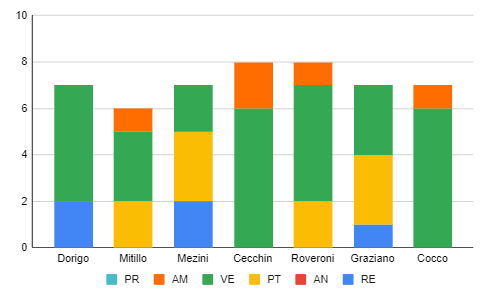
\includegraphics[width=0.7\linewidth]{../immagini/pdp/istogramma_progettazione_dettaglio_periodo3.png}
				\caption{Istogramma della ripartizione oraria durante il terzo periodo della fase di Progettazione di
					dettaglio e codifica}
			\end{center}
		\end{figure}
		\clearpage
		\subsubsection{Prospetto economico}\label{PreventivoFaseDiProgettazioneDiDettaglioECodificaProspettoEconomicoPeriodo3}
		\quad
		\def\tabularxcolumn#1{m{#1}}
		{\rowcolors{2}{RawSienna!90!RawSienna!20}{RawSienna!70!RawSienna!40}
			\begin{center}
				\renewcommand{\arraystretch}{1.4}
				\begin{tabularx}{7cm}{|X|c|c|}
					\hline
					\rowcolor{airforceblue}
					\textbf{Ruolo} & \textbf{Ore} & \textbf{Costo}\\
					\hline
					Responsabile & 5 & 150\euro\\
					\hline
					Amministratore & 5 & 100\euro\\
					\hline
					Analista & 0 & 0\euro\\
					\hline
					Progettista & 10 & 220\euro\\
					\hline
					Programmatore & 0 & 0\euro\\
					\hline
					Verificatore & 30 & 450\euro\\
					\hline
					Totale & 50 & 920\euro\\
					\hline
				\end{tabularx}
				\captionof{table}{\textbf{Prospetto dei costi per ruolo nel terzo periodo della fase di Progettazione di dettaglio e codifica}}
			\end{center}

			Il seguente grafico a torta riassume i dati ottenuti:
			\begin{figure}[!ht]
				\begin{center}
					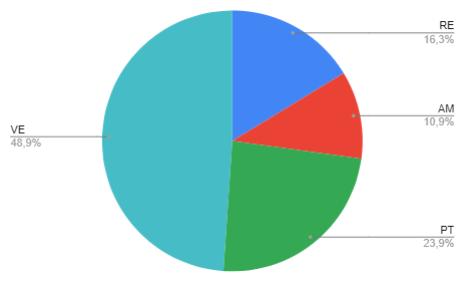
\includegraphics[width=0.8\linewidth]{../immagini/pdp/torta_progettazione_dettaglio_periodo3.png}
					\caption{Grafico a torta della ripartizione dei costi per ruolo del terzo periodo della fase di Progettazione e codifica}
				\end{center}
			\end{figure}

		\subsection{Prospetto complessivo}\label{PreventivoFaseDiProgettazioneDiDettaglioECodificaComplessivo}

			\subsubsection{Prospetto orario}\label{PreventivoFaseDiProgettazioneDiDettaglioECodificaProspettoOrario}
			In questa fase la distribuzione oraria è la seguente:
			\quad
			\def\tabularxcolumn#1{m{#1}}
			{\rowcolors{2}{RawSienna!90!RawSienna!20}{RawSienna!70!RawSienna!40}

				\begin{center}
					\renewcommand{\arraystretch}{1.4}
					\begin{tabularx}{\textwidth}{|X|c|c|c|c|c|c|c|}
						\hline
						\rowcolor{airforceblue}
						\textbf{Nominativo} & \textbf{Re} & \textbf{Am} & \textbf{An} & \textbf{Pt} & \textbf{Pr} & \textbf{Ve} & \textbf{Totale ore}\\
						\hline
						\textit{Andrea Dorigo} & 11 & 4 & 3 & 7 & 10 & 10 & 45\\
						\hline
						\textit{Margherita Mitillo} & 3 & 4 & 7 & 8 & 12 & 11 & 45\\
						\hline
						\textit{Igli Mezini} & 9 & 5 & 6 & 14 & 0 & 11 & 45\\
						\hline
						\textit{Andrea Cecchin} & 0 & 10 & 0 & 9 & 18 & 8 & 45\\
						\hline
						\textit{Emma Roveroni} & 3 & 5 & 2 & 10 & 14 & 11 & 45\\
						\hline
						\textit{Alfredo Graziano} & 9 & 6 & 6 & 11 & 0 & 13 & 45\\
						\hline
						\textit{Mattia Cocco} & 0 & 4 & 2 & 10 & 17 & 12 & 45\\
						\hline
						Totale ore ruolo & 35 & 38 & 26 & 69 & 71 & 76 & 315\\
						\hline
					\end{tabularx}
					\captionof{table}{\textbf{Distribuzione delle ore durante la Progettazione di dettaglio e codifica}}
				\end{center}
				Il seguente istogramma riassume i dati ottenuti:
				\begin{figure}[!h]
					\begin{center}
						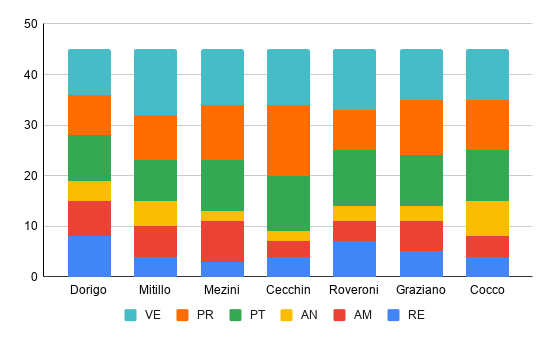
\includegraphics[width=0.7\linewidth]{../immagini/pdp/istogramma_progettazione_dettaglio.png}
						\caption{Istogramma della ripartizione oraria durante la Progettazione di
							dettaglio e codifica}
					\end{center}
				\end{figure}
				\clearpage
				\subsubsection{Prospetto economico}\label{PreventivoFaseDiProgettazioneDiDettaglioECodificaProspettoEconomico}
				\quad
				\def\tabularxcolumn#1{m{#1}}
				{\rowcolors{2}{RawSienna!90!RawSienna!20}{RawSienna!70!RawSienna!40}
					\begin{center}
						\renewcommand{\arraystretch}{1.4}
						\begin{tabularx}{7cm}{|X|c|c|}
							\hline
							\rowcolor{airforceblue}
							\textbf{Ruolo} & \textbf{Ore} & \textbf{Costo}\\
							\hline
							Responsabile & 35 & 1050\euro\\
							\hline
							Amministratore & 38 & 760\euro\\
							\hline
							Analista & 26 & 650\euro\\
							\hline
							Progettista & 69 & 1518\euro\\
							\hline
							Programmatore & 71 & 1065\euro\\
							\hline
							Verificatore & 76 & 1140\euro\\
							\hline
							Totale & 315 & 6183\euro\\
							\hline
						\end{tabularx}
						\captionof{table}{\textbf{Prospetto dei costi per ruolo nel periodo di Progettazione di dettaglio e codifica}}
					\end{center}

					Il seguente grafico a torta riassume i dati ottenuti:
					\begin{figure}[!ht]
						\begin{center}
							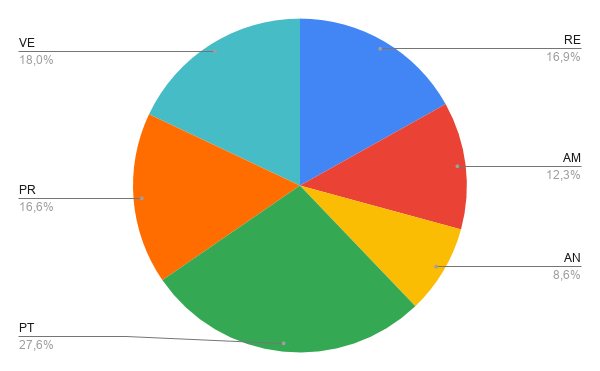
\includegraphics[width=0.8\linewidth]{../immagini/pdp/torta_progettazione_dettaglio.png}
							\caption{Grafico a torta della ripartizione dei costi per ruolo nella fase di Progettazione
								di dettaglio e codifica}
						\end{center}
					\end{figure}

\section{Fase di Validazione e collaudo}\label{PreventivoFaseDiProgettazionediValidazioneECollaudo}

% \subsection{Primo periodo}\label{PreventivoFaseDiProgettazionediValidazioneECollaudoPrimoPeriodo}
\subsection{Prospetto delle ore degli incrementi 12, 13 e 14}\label{PreventivoFaseDiProgettazionediValidazioneECollaudoIncrementi12-13-14}
Di seguito riportiamo la previsione delle ore che ciascun incremento necessita, relativamente agli incrementi 12, 13 e 14.
\quad
\def\tabularxcolumn#1{m{#1}}
{\rowcolors{2}{RawSienna!90!RawSienna!20}{RawSienna!70!RawSienna!40}

	\begin{center}
		\renewcommand{\arraystretch}{1.4}
		\begin{tabularx}{\textwidth}{|X|c|c|c|c|c|c|c|}
			\hline
			\rowcolor{airforceblue}
			\textbf{Incremento} & \textbf{Re} & \textbf{Am} & \textbf{An} & \textbf{Pt} & \textbf{Pr} & \textbf{Ve} & \textbf{Totale ore}\\
			\hline
			\textit{Incremento 12} & 2 & 3 & 0 & 0 & 14 & 0 & 19\\
			\hline
			\textit{Incremento 13} & 1 & 2 & 0 & 0 & 0 & 10 & 13\\
			\hline
			\textit{Incremento 14} & 2 & 3 & 0 & 0 & 0 & 13 & 18\\
			\hline
			Totale ore ruolo & 5 & 8 & 0 & 0 & 14 & 23 & 50\\
			\hline
		\end{tabularx}
		\captionof{table}{\textbf{Prospetto delle ore degli incrementi 12, 13 e 14 della fase di Validazione e Collaudo}}
	\end{center}

\subsubsection{Prospetto orario}\label{PreventivoFaseDiProgettazionediValidazioneECollaudoIncrementi12-13-14ProspettoOrario}
Per questi tre incrementi la distribuzione oraria tra i componenti del gruppo sarà la seguente:

\quad
\def\tabularxcolumn#1{m{#1}}
{\rowcolors{2}{RawSienna!90!RawSienna!20}{RawSienna!70!RawSienna!40}

	\begin{center}
		\renewcommand{\arraystretch}{1.4}
		\begin{tabularx}{\textwidth}{|X|c|c|c|c|c|c|c|}
			\hline
			\rowcolor{airforceblue}
			\textbf{Nominativo} & \textbf{Re} & \textbf{Am} & \textbf{An} & \textbf{Pt} & \textbf{Pr} & \textbf{Ve} & \textbf{Totale ore}\\
			\hline
			\textit{Andrea Dorigo} & 2 & 0 & 0 & 0 & 0 & 6 & 8\\
			\hline
			\textit{Margherita Mitillo} & 0 & 3 & 0 & 0 & 2 & 3 & 8\\
			\hline
			\textit{Igli Mezini} & 2 & 0 & 0 & 0 & 2 & 2 & 6\\
			\hline
			\textit{Andrea Cecchin} & 0 & 3 & 0 & 0 & 2 & 3 & 8\\
			\hline
			\textit{Emma Roveroni} & 0 & 2 & 0 & 0 & 2 & 3 & 7\\
			\hline
			\textit{Alfredo Graziano} & 1 & 0 & 0 & 0 & 2 & 3 & 6\\
			\hline
			\textit{Mattia Cocco} & 0 & 0 & 0 & 0 & 4 & 3 & 7\\
			\hline
			Totale ore ruolo & 5 & 8 & 0 & 0 & 14 & 23 & 50\\
			\hline
		\end{tabularx}
		\captionof{table}{\textbf{Distribuzione oraria degli incrementi 12, 13 e 14 della fase di Validazione e Collaudo}}
	\end{center}

Il seguente istogramma riassume i dati ottenuti:
\begin{figure}[!h]
	\begin{center}
		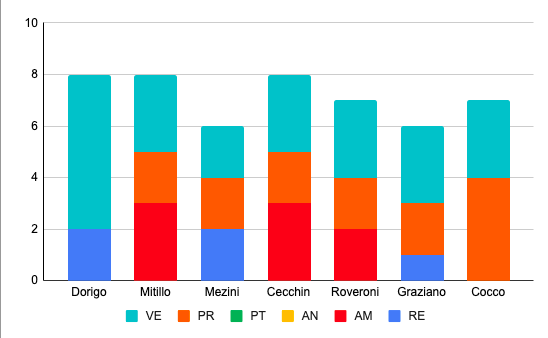
\includegraphics[width=0.7\linewidth]{../immagini/pdp/istogramma_validazione_collaudo_periodo1.png}
		\caption{Istogramma della ripartizione oraria durante gli incrementi 12, 13 e 14 della fase di Validazione e Collaudo}
	\end{center}
\end{figure}
\clearpage

\subsubsection{Prospetto economico}\label{PreventivoFaseDiProgettazionediValidazioneECollaudoIncrementi12-13-14ProspettoEconomico}
\quad
\def\tabularxcolumn#1{m{#1}}
{\rowcolors{2}{RawSienna!90!RawSienna!20}{RawSienna!70!RawSienna!40}
	\begin{center}
		\renewcommand{\arraystretch}{1.4}
		\begin{tabularx}{7cm}{|X|c|c|}
			\hline
			\rowcolor{airforceblue}
			\textbf{Ruolo} & \textbf{Ore} & \textbf{Costo}\\
			\hline
			Responsabile & 5 & 150\euro\\
			\hline
			Amministratore & 8 & 160\euro\\
			\hline
			Analista & 0 & 0\euro\\
			\hline
			Progettista & 0 & 0\euro\\
			\hline
			Programmatore & 14 & 210\euro\\
			\hline
			Verificatore & 23 & 345\euro\\
			\hline
			Totale & 50 & 865\euro\\
			\hline
		\end{tabularx}
		\captionof{table}{\textbf{Prospetto dei costi per ruolo per gli incrementi 12, 13 e 14 della fase di Validazione e collaudo}}
	\end{center}

	Il seguente grafico a torta riassume i dati ottenuti:
	\begin{figure}[!ht]
		\begin{center}
			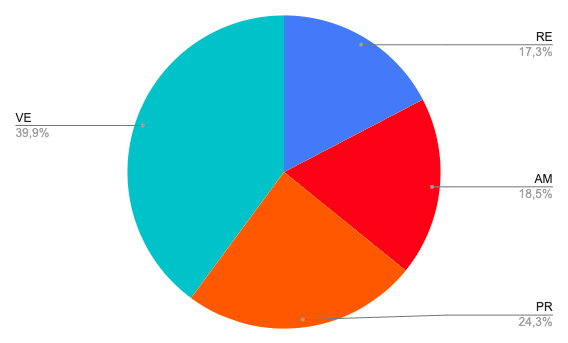
\includegraphics[width=0.8\linewidth]{../immagini/pdp/torta_validazione_collaudo_periodo1.png}
			\caption{Grafico a torta della ripartizione dei costi per ruolo del per gli incrementi 12, 13 e 14 della fase di Validazione e Collaudo}
		\end{center}
	\end{figure}

% \subsection{Secondo periodo}\label{PreventivoFaseDiProgettazionediValidazioneECollaudoSecondoPeriodo}
\subsection{Prospetto delle ore degli incrementi 15 e 16}\label{PreventivoFaseDiProgettazionediValidazioneECollaudoIncrementi15-16}
Di seguito riportiamo la previsione delle ore che ciascun incremento necessita, relativamente agli incrementi 15 e 16.
\quad
\def\tabularxcolumn#1{m{#1}}
{\rowcolors{2}{RawSienna!90!RawSienna!20}{RawSienna!70!RawSienna!40}

	\begin{center}
		\renewcommand{\arraystretch}{1.4}
		\begin{tabularx}{\textwidth}{|X|c|c|c|c|c|c|c|}
			\hline
			\rowcolor{airforceblue}
			\textbf{Incremento} & \textbf{Re} & \textbf{Am} & \textbf{An} & \textbf{Pt} & \textbf{Pr} & \textbf{Ve} & \textbf{Totale ore}\\
			\hline
			\textit{Incremento 15} & 3 & 7 & 0 & 0 & 24 & 0 & 34\\
			\hline
			\textit{Incremento 16} & 8 & 6 & 0 & 0 & 0 & 37 & 51\\
			\hline
			Totale ore ruolo & 11 & 13 & 0 & 0 & 24 & 37 & 85\\
			\hline
		\end{tabularx}
		\captionof{table}{\textbf{Prospetto delle ore degli incrementi degli intervalli 15 e 16 della fase di Validazione e Collaudo}}
	\end{center}

	\subsubsection{Prospetto orario}\label{PreventivoFaseDiProgettazionediValidazioneECollaudoIncrementi15-16ProspettoOrario}
	Per gli incrementi 15 e 16 la distribuzione oraria tra i componenti del gruppo sarà la seguente:

	\quad
	\def\tabularxcolumn#1{m{#1}}
	{\rowcolors{2}{RawSienna!90!RawSienna!20}{RawSienna!70!RawSienna!40}

		\begin{center}
			\renewcommand{\arraystretch}{1.4}
			\begin{tabularx}{\textwidth}{|X|c|c|c|c|c|c|c|}
				\hline
				\rowcolor{airforceblue}
				\textbf{Nominativo} & \textbf{Re} & \textbf{Am} & \textbf{An} & \textbf{Pt} & \textbf{Pr} & \textbf{Ve} & \textbf{Totale ore}\\
				\hline
				\textit{Andrea Dorigo} & 3 & 1 & 0 & 0 & 3 & 4 & 11\\
				\hline
				\textit{Margherita Mitillo} & 1 & 3 & 0 & 0 & 2 & 6 & 12\\
				\hline
				\textit{Igli Mezini} & 2 & 3 & 0 & 0 & 3 & 7 & 15\\
				\hline
				\textit{Andrea Cecchin} & 0 & 2 & 0 & 0 & 5 & 5 & 12\\
				\hline
				\textit{Emma Roveroni} & 2 & 0 & 0 & 0 & 4 & 4 & 10\\
				\hline
				\textit{Alfredo Graziano} & 3 & 2 & 0 & 0 & 3 & 7 & 15\\
				\hline
				\textit{Mattia Cocco} & 0 & 2 & 0 & 0 & 4 & 4 & 10\\
				\hline
				Totale ore ruolo & 11 & 13 & 0 & 0 & 24 & 37 & 85\\
				\hline
			\end{tabularx}
			\captionof{table}{\textbf{Distribuzione oraria degli incrementi 15 e 16 della fase di Validazione e Collaudo}}
		\end{center}

		Il seguente istogramma riassume i dati ottenuti:
		\begin{figure}[!h]
			\begin{center}
				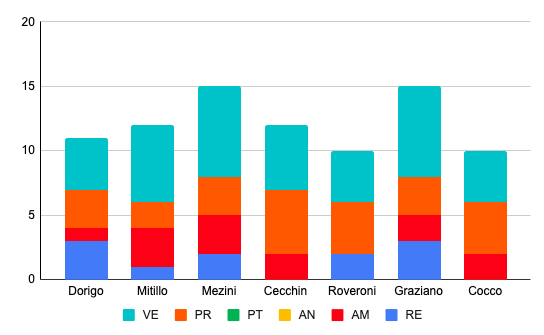
\includegraphics[width=0.7\linewidth]{../immagini/pdp/istogramma_validazione_collaudo_periodo2.png}
				\caption{Istogramma della ripartizione oraria durante gli incrementi 15 e 16 della fase di Validazione e Collaudo}
			\end{center}
		\end{figure}
		\clearpage

		\subsubsection{Prospetto economico}\label{PreventivoFaseDiProgettazionediValidazioneECollaudoIncrementi15-16ProspettoEconomico}
		\quad
		\def\tabularxcolumn#1{m{#1}}
		{\rowcolors{2}{RawSienna!90!RawSienna!20}{RawSienna!70!RawSienna!40}
			\begin{center}
				\renewcommand{\arraystretch}{1.4}
				\begin{tabularx}{7cm}{|X|c|c|}
					\hline
					\rowcolor{airforceblue}
					\textbf{Ruolo} & \textbf{Ore} & \textbf{Costo}\\
					\hline
					Responsabile & 11 & 330\euro\\
					\hline
					Amministratore & 13 & 260\euro\\
					\hline
					Analista & 0 & 0\euro\\
					\hline
					Progettista & 0 & 0\euro\\
					\hline
					Programmatore & 24 & 360\euro\\
					\hline
					Verificatore & 37 & 555\euro\\
					\hline
					Totale & 85 & 1505\euro\\
					\hline
				\end{tabularx}
				\captionof{table}{\textbf{Prospetto dei costi per ruolo degli incrementi 15 e 16 della fase di Validazione e collaudo}}
			\end{center}

			Il seguente grafico a torta riassume i dati ottenuti:
			\begin{figure}[!ht]
				\begin{center}
					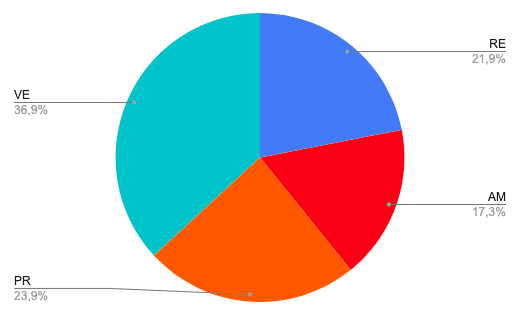
\includegraphics[width=0.8\linewidth]{../immagini/pdp/torta_validazione_collaudo_periodo2.png}
					\caption{Grafico a torta della ripartizione dei costi per ruolo degli incrementi 15 e 16 della fase di Validazione e Collaudo}
				\end{center}
			\end{figure}

% \subsection{Terzo periodo}\label{PreventivoFaseDiProgettazionediValidazioneECollaudoTerzoPeriodo}
\subsection{Prospetto delle ore degli incrementi 17 e 18}\label{PreventivoFaseDiProgettazionediValidazioneECollaudoIncrementi17-18}
Di seguito riportiamo la previsione delle ore che gli incrementi 17 e 18 necessitano:
\quad
\def\tabularxcolumn#1{m{#1}}
{\rowcolors{2}{RawSienna!90!RawSienna!20}{RawSienna!70!RawSienna!40}

	\begin{center}
		\renewcommand{\arraystretch}{1.4}
		\begin{tabularx}{\textwidth}{|X|c|c|c|c|c|c|c|}
			\hline
			\rowcolor{airforceblue}
			\textbf{Incremento} & \textbf{Re} & \textbf{Am} & \textbf{An} & \textbf{Pt} & \textbf{Pr} & \textbf{Ve} & \textbf{Totale ore}\\
			\hline
			\textit{Incremento 17} & 3 & 2 & 0 & 0 & 14 & 0 & 19\\
			\hline
			\textit{Incremento 18} & 2 & 5 & 0 & 0 & 14 & 0 & 21\\
			\hline
			Totale ore ruolo & 5 & 7 & 0 & 0 & 28 & 0 & 40\\
			\hline
		\end{tabularx}
		\captionof{table}{\textbf{Prospetto delle ore degli incrementi 17 e 18 della fase di Validazione e Collaudo}}
	\end{center}

	\subsubsection{Prospetto orario}\label{PreventivoFaseDiProgettazionediValidazioneECollaudoIncrementi17-18ProspettoOrario}
	Per questi incrementi la distribuzione oraria tra i componenti del gruppo sarà la seguente:

	\quad
	\def\tabularxcolumn#1{m{#1}}
	{\rowcolors{2}{RawSienna!90!RawSienna!20}{RawSienna!70!RawSienna!40}

		\begin{center}
			\renewcommand{\arraystretch}{1.4}
			\begin{tabularx}{\textwidth}{|X|c|c|c|c|c|c|c|}
				\hline
				\rowcolor{airforceblue}
				\textbf{Nominativo} & \textbf{Re} & \textbf{Am} & \textbf{An} & \textbf{Pt} & \textbf{Pr} & \textbf{Ve} & \textbf{Totale ore}\\
				\hline
				\textit{Andrea Dorigo} & 2 & 0 & 0 & 0 & 4 & 0 & 6\\
				\hline
				\textit{Margherita Mitillo} & 0 & 2 & 0 & 0 & 3 & 0 & 5\\
				\hline
				\textit{Igli Mezini} & 2 & 0 & 0 & 0 & 2 & 0 & 4\\
				\hline
				\textit{Andrea Cecchin} & 0 & 2 & 0 & 0 & 3 & 0 & 5\\
				\hline
				\textit{Emma Roveroni} & 0 & 1 & 0 & 0 & 7 & 0 & 8\\
				\hline
				\textit{Alfredo Graziano} & 1 & 0 & 0 & 0 & 3 & 0 & 4\\
				\hline
				\textit{Mattia Cocco} & 0 & 2 & 0 & 0 & 6 & 0 & 8\\
				\hline
				Totale ore ruolo & 5 & 7 & 0 & 0 & 28 & 0 & 40\\
				\hline
			\end{tabularx}
			\captionof{table}{\textbf{Distribuzione oraria degli incrementi 17 e 18 della fase di Validazione e Collaudo}}
		\end{center}

		Il seguente istogramma riassume i dati ottenuti:
		\begin{figure}[!h]
			\begin{center}
				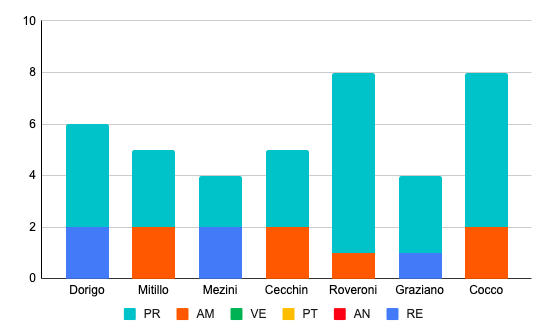
\includegraphics[width=0.7\linewidth]{../immagini/pdp/istogramma_validazione_collaudo_periodo3.png}
				\caption{Istogramma della ripartizione oraria durante gli incrementi 17 e 18 della fase di Validazione e Collaudo}
			\end{center}
		\end{figure}
		\clearpage

		\subsubsection{Prospetto economico}\label{PreventivoFaseDiProgettazionediValidazioneECollaudoIncrmenti17-18ProspettoEconomico}
		\quad
		\def\tabularxcolumn#1{m{#1}}
		{\rowcolors{2}{RawSienna!90!RawSienna!20}{RawSienna!70!RawSienna!40}
			\begin{center}
				\renewcommand{\arraystretch}{1.4}
				\begin{tabularx}{7cm}{|X|c|c|}
					\hline
					\rowcolor{airforceblue}
					\textbf{Ruolo} & \textbf{Ore} & \textbf{Costo}\\
					\hline
					Responsabile & 5 & 150\euro\\
					\hline
					Amministratore & 7 & 140\euro\\
					\hline
					Analista & 0 & 0\euro\\
					\hline
					Progettista & 0 & 0\euro\\
					\hline
					Programmatore & 28 & 420\euro\\
					\hline
					Verificatore & 0 & 0\euro\\
					\hline
					Totale & 40 & 710\euro\\
					\hline
				\end{tabularx}
				\captionof{table}{\textbf{Prospetto dei costi per ruolo negli incrementi 17 e 18 della fase di Validazione e collaudo}}
			\end{center}

			Il seguente grafico a torta riassume i dati ottenuti:
			\begin{figure}[!ht]
				\begin{center}
					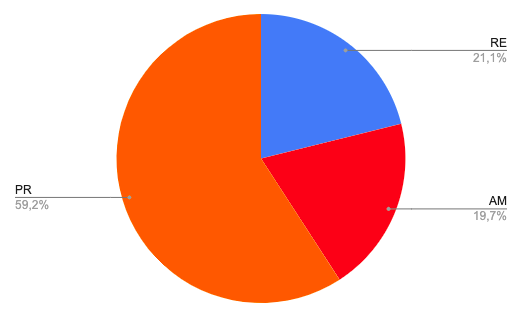
\includegraphics[width=0.8\linewidth]{../immagini/pdp/torta_validazione_collaudo_periodo3.png}
					\caption{Grafico a torta della ripartizione dei costi per ruolo degli incrementi 17 e 18 della fase di Validazione e Collaudo}
				\end{center}
			\end{figure}

\subsection{Prospetto complessivo}\label{PreventivoFaseValidazioneCollaudoComplessivo}
\subsubsection{Prospetto orario}\label{PreventivoFaseValidazioneCollaudoComplessivoProspettoOrario}
La distribuzione oraria totale di questa fase è la seguente:
\quad
\def\tabularxcolumn#1{m{#1}}
{\rowcolors{2}{RawSienna!90!RawSienna!20}{RawSienna!70!RawSienna!40}

	\begin{center}
		\renewcommand{\arraystretch}{1.4}
		\begin{tabularx}{\textwidth}{|X|c|c|c|c|c|c|c|}
			\hline
			\rowcolor{airforceblue}
			\textbf{Nominativo} & \textbf{Re} & \textbf{Am} & \textbf{An} & \textbf{Pt} & \textbf{Pr} & \textbf{Ve} & \textbf{Totale ore}\\
			\hline
			\textit{Andrea Dorigo} & 7 & 1 & 0 & 0 & 7 & 10 & 25\\
			\hline
			\textit{Margherita Mitillo} & 1 & 8 & 0 & 0 & 7 & 9 & 25\\
			\hline
			\textit{Igli Mezini} & 6 & 3 & 0 & 0 & 7 & 9 & 25\\
			\hline
			\textit{Andrea Cecchin} & 0 & 7 & 0 & 0 & 10 & 8 & 25\\
			\hline
			\textit{Emma Roveroni} & 2 & 3 & 0 & 0 & 13 & 7 & 25\\
			\hline
			\textit{Alfredo Graziano} & 5 & 2 & 0 & 0 & 8 & 10 & 25\\
			\hline
			\textit{Mattia Cocco} & 0 & 4 & 0 & 0 & 14 & 7 & 25\\
			\hline
			Totale ore ruolo & 21 & 28 & 0 & 0 & 66 & 60 & 175\\
			\hline
		\end{tabularx}
	\captionof{table}{\textbf{Distribuzione delle ore totali durante la fase di Validazione e collaudo}}
	\end{center}
Il seguente istogramma riassume i dati ottenuti:
\begin{figure}[!ht]
	\begin{center}
		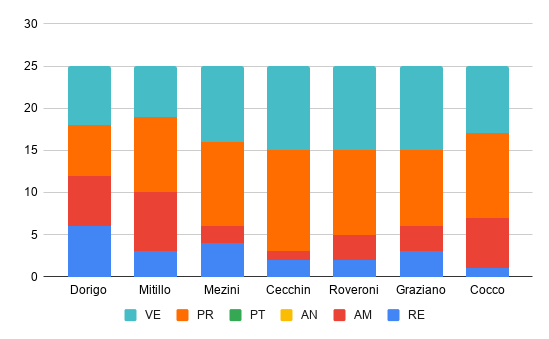
\includegraphics[width=0.7\linewidth]{../immagini/pdp/istogramma_validazione.png}
		\caption{Istogramma della ripartizione oraria durante la fase di Validazione e
			collaudo}
	\end{center}
\end{figure}
\clearpage
\subsubsection{Prospetto economico}\label{PreventivoFaseValidazioneCollaudoComplessivooProspettoEconomico}
\quad
\def\tabularxcolumn#1{m{#1}}
{\rowcolors{2}{RawSienna!90!RawSienna!20}{RawSienna!70!RawSienna!40}
	\begin{center}
		\renewcommand{\arraystretch}{1.4}
		\begin{tabularx}{7cm}{|X|c|c|}
			\hline
			\rowcolor{airforceblue}
			\textbf{Ruolo} & \textbf{Ore} & \textbf{Costo}\\
			\hline
			Responsabile & 21 & 630\euro\\
			\hline
			Amministratore & 28 & 560\euro\\
			\hline
			Analista & 0 & 0\euro\\
			\hline
			Progettista & 0 & 0\euro\\
			\hline
			Programmatore & 66 & 990\euro\\
			\hline
			Verificatore & 60 & 900\euro\\
			\hline
			Totale & 175 & 3080\euro\\
			\hline
		\end{tabularx}
	\captionof{table}{\textbf{Prospetto dei costi per ruolo nella fase di Validazione e collaudo}}
	\end{center}

Il seguente grafico a torta riassume i dati ottenuti:
\begin{figure}[!ht]
	\begin{center}
		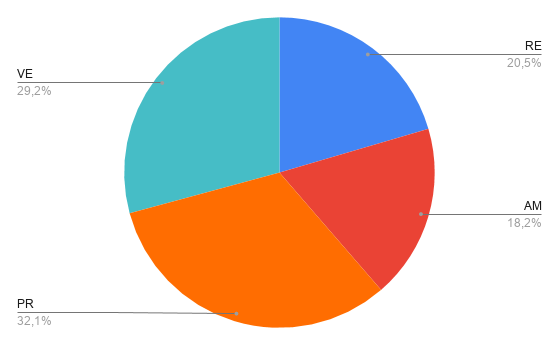
\includegraphics[width=0.8\linewidth]{../immagini/pdp/torta_validazione.png}
		\caption{Grafico a torta della ripartizione dei costi per ruolo della fase di Validazione e Collaudo}
	\end{center}
\end{figure}

\section{Riepilogo}\label{PreventivoRiepilogo}

\subsection{Ore totali}\label{PreventivoRiepilogoOreTotali}

\subsubsection{Suddivisione lavoro}\label{PreventivoRiepilogoOreTotaliSuddivisioneDelLavoro}
Nella seguente tabella vengono riportate il totale delle ore del progetto, sono presenti sia le ore di investimento, sia quelle rendicontate a carico del committente$_G$.
\quad
\def\tabularxcolumn#1{m{#1}}
{\rowcolors{2}{RawSienna!90!RawSienna!20}{RawSienna!70!RawSienna!40}

	\begin{center}
		\renewcommand{\arraystretch}{1.4}
		\begin{tabularx}{\textwidth}{|X|c|c|c|c|c|c|c|}
			\hline
			\rowcolor{airforceblue}
			\textbf{Nominativo} & \textbf{Re} & \textbf{Am} & \textbf{An} & \textbf{Pt} & \textbf{Pr} & \textbf{Ve} & \textbf{Totale ore}\\
			\hline
			\textit{Andrea Dorigo} & 33 & 17 & 8 & 23 & 21 & 32 & 134\\
			\hline
			\textit{Margherita Mitillo} & 17 & 24 & 23 & 20 & 19 & 31 & 134\\
			\hline
			\textit{Igli Mezini} & 23 & 17 & 22 & 22 & 10 & 40 & 134\\
			\hline
			\textit{Andrea Cecchin} & 13 & 31 & 15 & 19 & 30 & 26 & 134\\
			\hline
			\textit{Emma Roveroni} & 9 & 21 & 13 & 24 & 27 & 40 & 134\\
			\hline
			\textit{Alfredo Graziano} & 17 & 22 & 25 & 26 & 10 & 34 & 134\\
			\hline
			\textit{Mattia Cocco} & 8 & 19 & 17 & 21 & 32 & 37 & 134\\
			\hline
		\end{tabularx}
	\captionof{table}{\textbf{Distribuzione delle ore totali di investimento e rendicontate}}
	\end{center}

Il seguente istogramma riassume i dati ottenuti:
\begin{figure}[!h]
	\begin{center}
		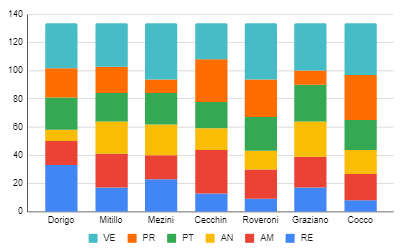
\includegraphics[width=0.65\linewidth]{../immagini/pdp/istogramma_suddivisione_lavoro1.png}
		\caption{Istogramma della ripartizione oraria totali di investimento e rendicontate}
	\end{center}
\end{figure}

\subsubsection{Prospetto economico}\label{PreventivoRiepilogoOreTotaliProspettoEconomico}
I costi da affrontare per ogni ruolo sono:
\quad
\def\tabularxcolumn#1{m{#1}}
{\rowcolors{2}{RawSienna!90!RawSienna!20}{RawSienna!70!RawSienna!40}
	\begin{center}
		\renewcommand{\arraystretch}{1.4}
		\begin{tabularx}{7cm}{|X|c|c|}
			\hline
			\rowcolor{airforceblue}
			\textbf{Ruolo} & \textbf{Ore} & \textbf{Costo}\\
			\hline
			Responsabile & 118 & 3540\euro\\
			\hline
			Amministratore & 153 & 3060\euro\\
			\hline
			Analista & 123 & 3075\euro\\
			\hline
			Progettista & 155 & 3410\euro\\
			\hline
			Programmatore & 149 & 2235\euro\\
			\hline
			Verificatore & 240 & 3600\euro\\
			\hline
			Totale & 938 & 18920\euro\\
			\hline
		\end{tabularx}
	\captionof{table}{\textbf{Prospetto dei costi totali delle ore totali di investimento e rendicontate}}
	\end{center}

Il seguente grafico a torta riassume i dati ottenuti:
\begin{figure}[!ht]
	\begin{center}
		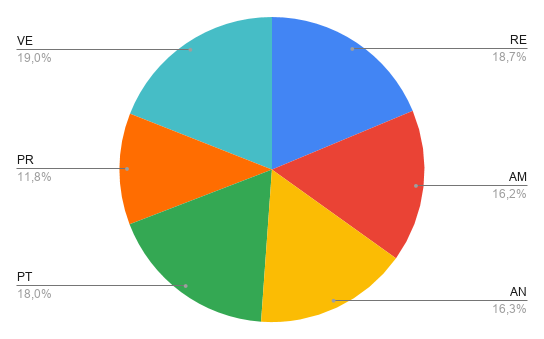
\includegraphics[width=0.8\linewidth]{../immagini/pdp/torta_suddvisione_lavoro.png}
		\caption{Grafico a torta della ripartizione dei costi per ruolo totali di investimento e
			rendicontate}
	\end{center}
\end{figure}

\subsection{Ore rendicontate}\label{PreventivoRiepilogoOreRendicontate}

\subsubsection{Suddivisione lavoro}\label{PreventivoRiepilogoOreRendicontateSuddivisioneLavoro}
Le ore rendicontate sono riportate nella seguente tabella:
\quad
\def\tabularxcolumn#1{m{#1}}
{\rowcolors{2}{RawSienna!90!RawSienna!20}{RawSienna!70!RawSienna!40}

	\begin{center}
		\renewcommand{\arraystretch}{1.4}
		\begin{tabularx}{\textwidth}{|X|c|c|c|c|c|c|c|}
			\hline
			\rowcolor{airforceblue}
			\textbf{Nominativo} & \textbf{Re} & \textbf{Am} & \textbf{An} & \textbf{Pt} & \textbf{Pr} & \textbf{Ve} & \textbf{Totale ore}\\
			\hline
			\textit{Andrea Dorigo} & 23 & 8 & 5 & 23 & 21 & 25 & 105\\
			\hline
			\textit{Margherita Mitillo} & 9 & 19 & 9 & 20 & 19 & 29 & 105\\
			\hline
			\textit{Igli Mezini} & 19 & 10 & 14 & 22 & 10 & 30 & 105\\
			\hline
			\textit{Andrea Cecchin} & 7 & 22 & 4 & 19 & 30 & 23 & 105\\
			\hline
			\textit{Emma Roveroni} & 6 & 15 & 6 & 24 & 27 & 27 & 105\\
			\hline
			\textit{Alfredo Graziano} & 16 & 10 & 15 & 26 & 10 & 28 & 105\\
			\hline
			\textit{Mattia Cocco} & 6 & 10 & 8 & 21 & 32 & 28 & 105\\
			\hline
		\end{tabularx}
	\captionof{table}{\textbf{Distribuzione delle ore rendicontate}}
	\end{center}
Il seguente istogramma riassume i dati ottenuti:
\begin{figure}[!ht]
	\begin{center}
		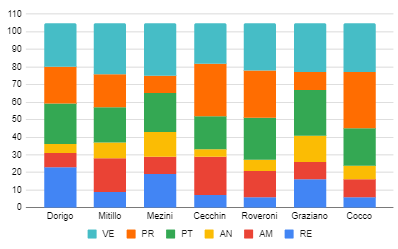
\includegraphics[width=0.8\linewidth]{../immagini/pdp/istogramma_rendicontate1.png}
		\caption{Istogramma della ripartizione oraria rendicontate}
	\end{center}
\end{figure}

\subsubsection{Prospetto economico}\label{PreventivoRiepilogoOreRendicontateProspettoEconomico}
Il totale rendicontato dei costi da affrontare per ogni ruolo è il seguenti:
\quad
\def\tabularxcolumn#1{m{#1}}
{\rowcolors{2}{RawSienna!90!RawSienna!20}{RawSienna!70!RawSienna!40}
	\begin{center}
		\renewcommand{\arraystretch}{1.4}
		\begin{tabularx}{7cm}{|X|c|c|}
			\hline
			\rowcolor{airforceblue}
			\textbf{Ruolo} & \textbf{Ore} & \textbf{Costo}\\
			\hline
			Responsabile & 86 & 2580\euro\\
			\hline
			Amministratore & 94 & 1880\euro\\
			\hline
			Analista & 61 & 1525\euro\\
			\hline
			Progettista & 155 & 3410\euro\\
			\hline
			Programmatore & 149 & 2235\euro\\
			\hline
			Verificatore & 190 & 2850\euro\\
			\hline
			Totale & 735 & 14480\euro\\
			\hline
		\end{tabularx}
	\captionof{table}{\textbf{Prospetto dei costi totali delle ore rendicontate}}
	\end{center}
Il seguente grafico a torta riassume i dati ottenuti:
\begin{figure}[!ht]
	\begin{center}
		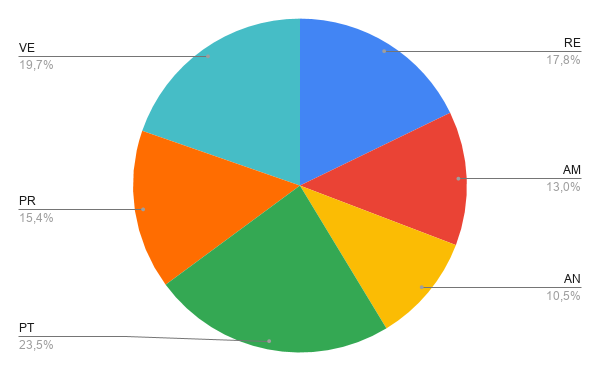
\includegraphics[width=0.8\linewidth]{../immagini/pdp/torta_rendicontate.png}
		\caption{Grafico a torta della ripartizione per ruolo delle ore rendicontate}
	\end{center}
\end{figure}
\subsection{Conclusioni}\label{PreventivoRiepilogoConclusioni}
Il costo totale del progetto considerando solamente le ore rendicontate è: 14480\euro.

\chapter{Consuntivo}\label{Consuntivo}
Di seguito vengono indicate le spese sostenute dal gruppo confrontandole con quanto preventivato. Il bilancio potrà essere:
\begin{itemize}
	\item positivo: la spesa effettiva è minore di quanto preventivato;
	\item pari: la spesa effettiva è uguale a quanto preventivato;
	\item negativo: la spesa effettiva è maggiore di quanto preventivato.
\end{itemize}
\section{Periodo di analisi}\label{ConsuntivoPeriodoDiAnalisi}
Le ore di lavoro che sono state sostenute durante la fase di analisi sono considerate come ore di investimento e per questo motivo esse non vengono rendicontate.
\quad
\def\tabularxcolumn#1{m{#1}}
{\rowcolors{2}{RawSienna!90!RawSienna!20}{RawSienna!70!RawSienna!40}
	\begin{center}
		\renewcommand{\arraystretch}{1.4}
		\begin{tabularx}{10cm}{|X|c|c|}
			\hline
			\rowcolor{airforceblue}
			\textbf{Ruolo} & \textbf{Ore} & \textbf{Costo}\\
			\hline
			Responsabile & 26(+0) & 780\euro(+0\euro)\\
			\hline
			Amministratore & 42(+0) & 840\euro(+0\euro)\\
			\hline
			Analista & 49(+15) & 1225\euro(+375\euro)\\
			\hline
			Progettista & 0(+0) & 0\euro(+0\euro)\\
			\hline
			Programmatore & 0(+0) & 0\euro(+0\euro)\\
			\hline
			Verificatore & 33(+10) & 495\euro(+150\euro)\\
			\hline
			\textbf{Totale Preventivo} & \textbf{150} & \textbf{3340\euro}\\
			\hline
			\textbf{Totale Consuntivo} & \textbf{175} & \textbf{3865\euro}\\
			\hline
			\textbf{Differenza} & \textbf{25} & \textbf{525\euro}
		\end{tabularx}
		\captionof{table}{\textbf{Consuntivo della fase di Analisi}}
	\end{center}

\subsection{Conclusioni}\label{ConsuntivoPeriodoDiAnalisiConclusioni}
Come emerso dalla tabella precedente, il bilancio risulta negativo in quanto il gruppo ha ritenuto necessario impiegare più tempo del previsto nei ruoli di \textit{Analista} e \textit{Verificatore}. I motivi di tale ritardo sono:
\begin{itemize}
	\item la complessità nell'individuazione dei requisiti;
	\item la grande quantità di lavoro nel revisionare i documenti. Infatti, trattandosi di un processo nuovo, ogni componente ha dovuto imparare a svolgerlo in maniera corretta, efficacie ed efficiente.
\end{itemize}

\subsection{Preventivo a finire}\label{ConsuntivoPeriodoDiAnalisiPreventivoAFinire}
Il preventivo a finire, nonostante in questa fase siano state necessarie più ore del previsto, è in linea con quanto descritto nella sezione precedente. Il gruppo non ritiene il surplus di 500\euro{} un problema in quanto le ore lavorative e i costi sostenuti in questa fase non verranno rendicontati. Per questo motivo il gruppo ha deciso di non prendere alcuna contromisura nella pianificazione futura.

\section{Periodo di consolidamento dei requisiti}\label{ConsuntivoPeriodoDiConsolidamentoDeiRequisiti}
Le ore di lavoro calcolate per questo periodo sono considerate come ore di investimento e, per tale motivo, non vengono rendicontate.

\quad
\def\tabularxcolumn#1{m{#1}}
{\rowcolors{2}{RawSienna!90!RawSienna!20}{RawSienna!70!RawSienna!40}
	\begin{center}
		\renewcommand{\arraystretch}{1.4}
		\begin{tabularx}{10cm}{|X|c|c|}
			\hline
			\rowcolor{airforceblue}
			\textbf{Ruolo} & \textbf{Ore} & \textbf{Costo}\\
			\hline
			Responsabile & 4(+0) & 120\euro(+0\euro)\\
			\hline
			Amministratore & 8(+0) & 160\euro(+0\euro)\\
			\hline
			Analista & 4(+0) & 100\euro(+0\euro)\\
			\hline
			Progettista & 0(+0) & 0\euro(+0\euro)\\
			\hline
			Programmatore & 0(+0) & 0\euro(+0\euro)\\
			\hline
			Verificatore & 8(0) & 120\euro(+0\euro)\\
			\hline
			\textbf{Totale Preventivo} & \textbf{24} & \textbf{500\euro}\\
			\hline
			\textbf{Totale Consuntivo} & \textbf{24} & \textbf{500\euro}\\
			\hline
			\textbf{Differenza} & \textbf{0} & \textbf{0\euro}
		\end{tabularx}
		\captionof{table}{\textbf{Consuntivo della fase di Consolidamento dei requisiti}}
	\end{center}

\subsection{Conclusioni}\label{ConsuntivoPeriodoDiConsolidamentoDeiRequisitiConclusioni}
Grazie al minor carico di lavoro, le ore preventivate sono state rispettate quindi non è presente alcuna differenza rispetto alle ore effettive di lavoro. Inoltre il gruppo è riuscito a procedere senza alcun problema con lo studio personale per lo svolgimento della fase successiva del lavoro.

\subsection{Preventivo a finire}\label{ConsuntivoPeriodoDiConsolidamentoDeiRequisitiPreventivoAFinire}
Poichè le ore di lavoro previste sono state rispettate, il preventivo a finire risulta coerente con quello previsto.

\section{Periodo di progettazione architetturale}\label{ConsuntivoPeriodoDiProgettazioneArchitetturale}

Il gruppo ha suddiviso questa fase in diversi periodi per organizzare al meglio il lavoro, di conseguenza il consuntivo viene analizzato in funzione di ogni sua parte.

\subsection{Primo periodo - dal 19-01-2021 al 15-02-2021}\label{ConsuntivoPeriodoDiProgettazioneArchitetturaleIncrementoEVerifica}

Le ore dedicate in questo periodo sono atte al completamento della fase di Incremento e Verifica descritta nella \S~\ref{PianificazioneProgettazioneArchitetturale} e a formazione personale sulle tecnologie da utilizzare per lo sviluppo della Technology Baseline$_{\scaleto{G}{3pt}}$.

\quad
\def\tabularxcolumn#1{m{#1}}
{\rowcolors{2}{RawSienna!90!RawSienna!20}{RawSienna!70!RawSienna!40}
	\begin{center}
		\renewcommand{\arraystretch}{1.4}
		\begin{tabularx}{10cm}{|X|c|c|}
			\hline
			\rowcolor{airforceblue}
			\textbf{Ruolo} & \textbf{Ore} & \textbf{Costo}\\
			\hline
			Responsabile & 7(+0) & 210\euro(+0\euro)\\
			\hline
			Amministratore & 7(+0) & 140\euro(+0\euro)\\
			\hline
			Analista & 8(+10) & 200\euro(+250\euro)\\
			\hline
			Progettista & 2(+0) & 44\euro(+0\euro)\\
			\hline
			Programmatore & 0(+0) & 0\euro(+0\euro)\\
			\hline
			Verificatore & 15(+10) & 225\euro(+150\euro)\\
			\hline
			\textbf{Totale Preventivo} & \textbf{39} & \textbf{819\euro}\\
			\hline
			\textbf{Totale Consuntivo} & \textbf{59} & \textbf{1219\euro}\\
			\hline
			\textbf{Differenza} & \textbf{20} & \textbf{400\euro}
		\end{tabularx}
		\captionof{table}{\textbf{Consuntivo del primo periodo}}
	\end{center}

\subsubsection{Conclusioni}
Come emerso dalla tabella precedente, il bilancio risulta negativo in quanto il gruppo ha ritenuto necessario impiegare più tempo del previsto nel ruolo di \textit{Verificatore} e di \textit{Analista}, per via l'esigenza di correggere alcuni errori sollevati in seguito alla Revisione dei Requisiti. 
%(voglio dire che abbiamo corretto i difetti gravi segnalati da tullio ed è per questo che il verificatore ha queste ore in più ma non so come dirlo in modo carino e formale)

\subsubsection{Preventivo a finire}
Il preventivo a finire presenta un surplus di 400\euro. Per questo motivo il gruppo ha deciso di tamponare il problema cercando di rispettare le ore preventivate nelle fasi successive in modo tale da non sforare troppo dal preventivo inizialmente previsto.

\subsection{Secondo periodo - dal 16-02-2021 al 04-03-2021 }\label{ConsuntivoPeriodoDiProgettazioneArchitetturaleTechnologyBaselinePrimoIncremento}

Le ore dedicate in questo periodo sono atte al completamento del primo incremento descritto nella  \S~\ref{PianificazioneProgettazioneArchitetturale}.

\quad
\def\tabularxcolumn#1{m{#1}}
{\rowcolors{2}{RawSienna!90!RawSienna!20}{RawSienna!70!RawSienna!40}
	\begin{center}
		\renewcommand{\arraystretch}{1.4}
		\begin{tabularx}{10cm}{|X|c|c|}
			\hline
			\rowcolor{airforceblue}
			\textbf{Ruolo} & \textbf{Ore} & \textbf{Costo}\\
			\hline
			Responsabile & 9(+0) & 270\euro(+0\euro)\\
			\hline
			Amministratore & 10(+0) & 200\euro(+0\euro)\\
			\hline
			Analista & 11(+0) & 275\euro(+0\euro)\\
			\hline
			Progettista & 54(+15) & 1188\euro(+330\euro)\\
			\hline
			Programmatore & 7(+0) & 105\euro(+0\euro)\\
			\hline
			Verificatore & 20(+0) & 300\euro(+0\euro)\\
			\hline
			\textbf{Totale Preventivo} & \textbf{111} & \textbf{2338\euro}\\
			\hline
			\textbf{Totale Consuntivo} & \textbf{126} & \textbf{2668\euro}\\
			\hline
			\textbf{Differenza} & \textbf{15} & \textbf{330\euro}
		\end{tabularx}
		\captionof{table}{\textbf{Consuntivo del secondo periodo}}
	\end{center}

\subsubsection{Conclusioni}
Come emerso dalla tabella precedente, il bilancio risulta negativo in quanto il gruppo ha ritenuto necessario impiegare più tempo del previsto nel ruolo di \textit{Progettista}. Il motivo di ciò è la mole di lavoro inaspettata che ha dovuto ricoprire questo ruolo per l'acerbità dei componenti riguardo alle tecnologie da utilizzare.

\subsubsection{Preventivo a finire}
Il preventivo a finire presenta un surplus di 330\euro. Per cercare di rientrare nelle ore prestabilite per le consegne successive, il gruppo ha deciso di organizzare meglio lo studio individuale di ognuno e di migliorare la comunicazione interna: in questo modo, quando emerge un problema, questo può essere risolto non dal singolo, che potrebbe impiegarci troppo tempo, ma dal gruppo.

\subsection{Terzo periodo - dal 05-03-2021 al 15-03-2021}\label{ConsuntivoPeriodoDiProgettazioneArchitetturaleTechnologyBaselineTerzoIncremento}

Le ore dedicate in questo periodo sono atte al completamento del secondo incremento descritto nella \S~\ref{PianificazioneProgettazioneArchitetturale}.

\quad
\def\tabularxcolumn#1{m{#1}}
{\rowcolors{2}{RawSienna!90!RawSienna!20}{RawSienna!70!RawSienna!40}
	\begin{center}
		\renewcommand{\arraystretch}{1.4}
		\begin{tabularx}{10cm}{|X|c|c|}
			\hline
			\rowcolor{airforceblue}
			\textbf{Ruolo} & \textbf{Ore} & \textbf{Costo}\\
			\hline
			Responsabile & 8(+0) & 240\euro(+0\euro)\\
			\hline
			Amministratore & 9(+0) & 180\euro(+0\euro)\\
			\hline
			Analista & 10(+0) & 250\euro(+0\euro)\\
			\hline
			Progettista & 30(+5) & 660\euro(+150\euro)\\
			\hline
			Programmatore & 5(+0) & 75\euro(+0\euro)\\
			\hline
			Verificatore & 19(+0) & 285\euro(+0\euro)\\
			\hline
			\textbf{Totale Preventivo} & \textbf{81} & \textbf{1690\euro}\\
			\hline
			\textbf{Totale Consuntivo} & \textbf{86} & \textbf{1840\euro}\\
			\hline
			\textbf{Differenza} & \textbf{5} & \textbf{150\euro}
		\end{tabularx}
		\captionof{table}{\textbf{Consuntivo del terzo periodo}}
	\end{center}

\subsubsection{Conclusioni}
Come emerso dalla tabella il bilancio risulta essere negativo in quanto il gruppo ha ritenuto necessario impiegare più tempo del previsto nel ruolo di \textit{Progettista} dovuto alla mole di lavoro legata al secondo incremento e alla conclusione dei documenti da presentare per la Revisione di Progettazione.

\subsubsection{Preventivo a finire}
Il preventivo a finire presenta un surplus di 150\euro. Per cercare di rientrare nelle ore prestabilite il gruppo ha lavorato in modo tale da avvantaggiarsi con il lavoro della fase successiva.

\subsection{Consuntivo complessivo delle fasi}\label{ConsuntivoPeriodoDiProgettazioneArchitetturaleConsuntivoComplessivoDelleFasi}

Nella tabella successiva viene descritto il calcolo delle ore totali di tutte le parti precedentemente descritte.

\quad
\def\tabularxcolumn#1{m{#1}}
{\rowcolors{2}{RawSienna!90!RawSienna!20}{RawSienna!70!RawSienna!40}
	\begin{center}
		\renewcommand{\arraystretch}{1.4}
		\begin{tabularx}{10cm}{|X|c|c|}
			\hline
			\rowcolor{airforceblue}
			\textbf{Ruolo} & \textbf{Ore} & \textbf{Costo}\\
			\hline
			Responsabile & 24(+0) & 720\euro(+0\euro)\\
			\hline
			Amministratore & 26(+0) & 520\euro(+0\euro)\\
			\hline
			Analista & 29(+10) & 725\euro(+250\euro)\\
			\hline
			Progettista & 86(+20) & 1892\euro(+440\euro)\\
			\hline
			Programmatore & 12(+0) & 180\euro(+0\euro)\\
			\hline
			Verificatore & 54(+10) & 810\euro(+150\euro)\\
			\hline
			\textbf{Totale Preventivo} & \textbf{231} & \textbf{4847\euro}\\
			\hline
			\textbf{Totale Consuntivo} & \textbf{271} & \textbf{5687\euro}\\
			\hline
			\textbf{Differenza} & \textbf{40} & \textbf{840\euro}
		\end{tabularx}
		\captionof{table}{\textbf{Consuntivo complessivo delle fasi}}
	\end{center}

\subsection{Conclusioni}\label{ConsuntivoPeriodoDiProgettazioneArchitetturaleConclusioni}
Il bilancio, come emerge dalla tabella precedente, risulta negativo poiché il gruppo ha ritenuto necessario impiegare più ore nei ruoli di \textit{Progettista},\textit{Verificatore} e \textit{Analista}. I motivi di tale ritardo sono:
\begin{itemize}
	\item il tempo impiegato per la correzione e l'aggiornamento dei documenti si è rivelato essere più di quello preventivato;
	\item trattandosi di un progetto complesso ed articolato, con tecnologie nuove ad ogni componente del gruppo, la parte di progettazione si è rivelata molto più complicata del previsto.
\end{itemize}

\subsection{Preventivo a finire}\label{ConsuntivoPeriodoDiProgettazioneArchitetturalePreventivoAFinire}
Il preventivo a finire risulta quindi con un surplus di 840\euro. Dalle analisi fatte riguardo ai preventivi a finire di ogni parte di questa fase il gruppo ha rilevato che:
\begin{itemize}
	\item deve essere presente un'organizzazione migliore nella verifica e validazione dei documenti;
	\item lo studio personale delle tecnologie deve essere più efficiente in modo da poter sviluppare in maniera più proficua;
	\item il miglioramento delle comunicazioni interne al gruppo può essere una parte fondamentale nella risoluzione di possibili problemi che emergono nel corso dello sviluppo del progetto.
\end{itemize}
Se ogni componente cerca di perseguire questi tre obiettivi il surplus presente in questo preventivo non risulterà un problema per l'ideazione del progetto. Inoltre per cercare di sopperire le ore aggiuntive il gruppo ha cercato di avanzare il più possibile con lo sviluppo dell'applicazione per non gravare troppo nelle fasi successive.
\chapter{Organigramma}\label{Organigramma}

\section{Redazione}\label{OrganigrammaRedazione}
\quad
\def\tabularxcolumn#1{m{#1}}
{\rowcolors{2}{RawSienna!90!RawSienna!20}{RawSienna!70!RawSienna!40}	
	\begin{center}
		\renewcommand{\arraystretch}{1.4}
		\begin{tabularx}{\textwidth}{|X|c|c|}
			\hline
			\rowcolor{airforceblue}
			\textbf{Nominativo} & \textbf{Data di Redazione} & \textbf{Firma}\\
			\hline
			Andrea Dorigo & 10-01-2021 & 
\includegraphics[width=0.2\linewidth]{../immagini/firme/firma_andrea_dorigo.png}\\
			\hline
			Margherita Mitillo & 10-01-2021 & 
\includegraphics[width=0.2\linewidth]{../immagini/firme/firma_margherita.png}\\
			\hline
			Mattia Cocco & 10-01-2021 &
\includegraphics[width=0.2\linewidth]{../immagini/firme/firma_mattia.png}\\
			\hline
			Igli Mezini & 10-01-2021 &
\includegraphics[width=0.3\linewidth]{../immagini/firme/firma_igli.png}\\
			\hline
		\end{tabularx}
		\captionof{table}{\textbf{Tabella dei nominativi addetti alla redazione}}
	\end{center}

\section{Approvazione}\label{OrganigrammaApprovazione}
\quad
\def\tabularxcolumn#1{m{#1}}
{\rowcolors{2}{RawSienna!90!RawSienna!20}{RawSienna!70!RawSienna!40}	
	\begin{center}
		\renewcommand{\arraystretch}{1.4}
		\begin{tabularx}{\textwidth}{|X|c|c|}
			\hline
			\rowcolor{airforceblue}
			\textbf{Nominativo} & \textbf{Data di Approvazione} & \textbf{Firma}\\
			\hline
			Andrea Dorigo & 11-01-2021 & 
\includegraphics[width=0.2\linewidth]{../immagini/firme/firma_andrea_dorigo.png}\\
			\hline
			Tullio Vardanega & &\\
			Riccardo Cardin & &\\
			\hline
		\end{tabularx}
		\captionof{table}{\textbf{Tabella dei nominativi addetti all'approvazione}}
	\end{center}
\clearpage
\section{Accettazione dei componenti}\label{OrganigrammaAccettazioneDeiComponenti}
\quad
\def\tabularxcolumn#1{m{#1}}
{\rowcolors{2}{RawSienna!90!RawSienna!20}{RawSienna!70!RawSienna!40}	
	\begin{center}
		\renewcommand{\arraystretch}{1.4}
		\begin{tabularx}{\textwidth}{|X|c|c|}
			\hline
			\rowcolor{airforceblue}
			\textbf{Nominativo} & \textbf{Data di Accettazione} & \textbf{Firma}\\
			\hline
			Andrea Dorigo & 10-01-2021 & 
\includegraphics[width=0.2\linewidth]{../immagini/firme/firma_andrea_dorigo.png}\\
			\hline
			Margherita Mitillo & 10-01-2021 & 
\includegraphics[width=0.2\linewidth]{../immagini/firme/firma_margherita.png}\\
			\hline
			Igli Mezini & 10-01-2021 &
\includegraphics[width=0.3\linewidth]{../immagini/firme/firma_igli.png}\\
			\hline
			Emma Roveroni & 10-01-2021 &
\includegraphics[width=0.2\linewidth]{../immagini/firme/firma_emma.png}\\
			\hline
			Mattia Cocco & 10-01-2021 &
\includegraphics[width=0.2\linewidth]{../immagini/firme/firma_mattia.png}\\
			\hline
			Alfredo Graziano & 10-01-2021 &
\includegraphics[width=0.2\linewidth]{../immagini/firme/firma_alfredo.png}\\
			\hline
			Andrea Cecchin & 10-01-2021 & 
\includegraphics[width=0.2\linewidth]{../immagini/firme/firma_andrea_c.png}\\
			\hline
		\end{tabularx}
		\captionof{table}{\textbf{Tabella dell'accettazione dei componenti}}
	\end{center}
\clearpage
\section{Componenti}\label{OrganigrammaComponenti}
\quad
\def\tabularxcolumn#1{m{#1}}
{\rowcolors{2}{RawSienna!90!RawSienna!20}{RawSienna!70!RawSienna!40}	
	\begin{center}
		\renewcommand{\arraystretch}{1.4}
		\begin{tabularx}{\textwidth}{|X|c|c|}
			\hline
			\rowcolor{airforceblue}
			\textbf{Nominativo} & \textbf{Matricola} & \textbf{Indirizzo di posta elettronica}\\
			\hline
			Andrea Dorigo & 1170610 & andrea.dorigo.3@studenti.unipd.it\\
			\hline
			Margherita Mitillo & 1098971 & margherita.mitillo@studenti.unipd\\
			\hline
			Igli Mezini & 1149009 & igli.mezini@studenti.unipd.it\\
			\hline
			Emma Roveroni & 1187275 & emma.roveroni@studenti.unipd.it\\
			\hline
			Mattia Cocco & 1096738 & mattia.cocco@studenti.unipd.it\\
			\hline
			Alfredo Graziano & 1144530 & alfredo.graziano@studenti.unipd.it\\
			\hline
			Andrea Cecchin & 1171050  & andrea.cecchin.3@studenti.unipd.it\\
			\hline
		\end{tabularx}
		\captionof{table}{\textbf{Tabella delle informazioni dei componenti}}
	\end{center}

%PER RENDERE PIÙ CHIARA LA STESURA DEI DOCUMENTI È MEGLIO LASCIARE SEPARATI IN FILE DIVERSI OGNI CAPITOLO

% \input{esempio} -- esempio di codice per inserire un nuovo capitolo

\end{document}

% \documentclass[a4paper,12pt]{report}
% \usepackage[utf8]{inputenc}
% \usepackage{graphicx}
% \usepackage{float}
% \usepackage{tabularx}
% \usepackage{makecell}
% \usepackage{titlesec}
% \usepackage{fancyhdr}
% \usepackage{lastpage}
% \usepackage{xurl}
% \usepackage{hyperref}
% \usepackage{geometry}
% \usepackage{color}
% \usepackage{microtype}
% \usepackage{enumerate}
% \usepackage{listings}
% \usepackage{tabularx}
% \usepackage[table,dvipsnames]{xcolor}
% \usepackage{caption}
% \captionsetup{labelformat=empty}
% \setcounter{tocdepth}{5}
% \setcounter{secnumdepth}{5} %SONO I DUE COMANDI PER AVERE LE SUBSUBSECTION NUMERATE E PRESENTI NELL'INDICE
% \renewcommand{\contentsname}{Indice} %QUESTO SERVE PER AVERE L'INDICE CON IL NOME CHE VOGLIO IO
% \renewcommand{\listfigurename}{Lista delle figure}
% \renewcommand{\listtablename}{Lista delle tabelle}
% \titleformat{\chapter}[display]
% {\normalfont\bfseries}{}{0pt}{\LARGE} %QUESTO SERVE PER AVERE SOLO IL NOME DEL CAPITOLO CHE VOGLIO IO
% \titlespacing*{\chapter}{0cm}{0cm}{0.2cm}
% \geometry{
% 	left=20mm,
% 	right=20mm,
% }
% \fancypagestyle{plain}{
% 	\fancyhf{}
% 	\lhead{
\includegraphics[width=3cm]{../immagini/minilogo.jpg}}
% 	\chead{}
% 	\rhead{\fontsize{12}{10}Piano di progetto}
% 	\lfoot{}
% 	\cfoot{\thepage\ di \pageref*{LastPage}}
% 	\rfoot{}
% }
%
% \definecolor{atomlightorange}{rgb}{0.88,0.76,0.55}
% \definecolor{atomdarkgrey}{RGB}{59,62,75}
%
% \usepackage{tikz}
%
% % set listings
% \lstset{%
%     basicstyle=\footnotesize\ttfamily\color{atomlightorange},
%     framesep=20pt,
% 		belowskip=10pt,
% 		aboveskip=10pt
% }
%
% % add frame environment
% \usepackage[%
%     framemethod=tikz,
%     skipbelow=8pt,
%     skipabove=13pt
% ]{mdframed}
% \mdfsetup{%
%     leftmargin=0pt,
%     rightmargin=0pt,
%     backgroundcolor=atomdarkgrey,
%     middlelinecolor=atomdarkgrey,
%     roundcorner=6
% }
%
% \usepackage{etoolbox}% >= v2.1 2011-01-03
% \BeforeBeginEnvironment{lstlisting}{\begin{mdframed}\vspace{-0.7em}}
% \AfterEndEnvironment{lstlisting}{\vspace{-0.5em}\end{mdframed}}
%
% % needed for \lstcapt
% \def\ifempty#1{\def\temparg{#1}\ifx\temparg\empty}
%
% % make new caption command for listings
% \usepackage{caption}
% \newcommand{\lstcapt}[2][]{%
%     \ifempty{#1}%
%         \captionof{lstlisting}{#2}%
%     \else%
%         \captionof{lstlisting}[#1]{#2}%
%     \fi%
%     \vspace{0.75\baselineskip}%
% }
%
% \hypersetup{
%     colorlinks=true,
%     linkcolor=black,
%     filecolor=black,
%     urlcolor=blue,
% 		citecolor=black,
% }
%
% \pagestyle{plain}
%
% \makeatletter
% 	 \def\thebibliography#1{\chapter*{Bibliografia\@mkboth
% 		 {Bibliografia}{Bibliografia}}\list
% 		 {[\arabic{enumi}]}{\settowidth\labelwidth{[#1]}\leftmargin\labelwidth
%  \advance\leftmargin\labelsep
%  \usecounter{enumi}}
%  \def\newblock{\hskip .11em plus .33em minus .07em}
%  \sloppy\clubpenalty4000\widowpenalty4000
%  \sfcode`\.=1000\relax}
% 	 \makeatother
%
% \newcolumntype{Y}{>{\centering\arraybackslash}X}
%
% \begin{document}
%
% \makeatletter
% \begin{titlepage}
%     \begin{center}
%     \vspace*{-5,0cm}
%     \author{Jawa Druids}
%     \title{Piano di progetto}
%     \date{} %LASCIARE QUESTO CAMPO VUOTO, SE LO TOLGO STAMPA LA DATA CORRENTE
%     
\includegraphics[width=0.7\linewidth]{../immagini/DRUIDSLOGO.jpg}\\[4ex]
%     {\huge \bfseries  \@title }\\[2ex]
%     {\LARGE  \@author}\\[50ex]
%     \vspace*{-8,0cm}
%     \begin{table}[H]
%         \centering
%         \begin{tabular}{c|c}
%             \textbf{Versione} & x.x.x \\
%             \textbf{Data approvazione} & xx-xx-xxxx\\
%             \textbf{Responsabile} & Nome Cognome\\
%             \textbf{Redattori} & Andrea Dorigo \\
%             \textbf{Verificatori} & Nome Cognome \\
%         %MAKECELL SERVE PER POI ANDARE A CAPO ALL'INTERNO DELLA CELLA
%             \textbf{Stato} & Redazione in corso\\
%             \textbf{Lista distribuzione} & \makecell{Jawa Druids \\ prof. Tullio Vardanega \\ prof. Riccardo Cardin \\ Sync Lab}\\
%             \textbf{Uso} & Esterno
%         \end{tabular}
%     \end{table}
% 					\vspace{.4cm}
% 	\hfill \break
%     \fontsize{17}{10}\textbf{Sommario}\\
% 		\vspace{.3cm}
%     Il presente documento contiene la pianificazione delle attività del gruppo Jawa Druids atte al soddisfacimento del capitolato \normalsize\textit{GDP: Gathering Detection Platform} di Sync Lab.
%     \end{center}
% \end{titlepage}
% \makeatother
%
% \quad
\begin{center}
	\LARGE\textbf{Registro delle modifiche}
\end{center}

\def\tabularxcolumn#1{m{#1}}
{\rowcolors{2}{RawSienna!90!RawSienna!20}{RawSienna!70!RawSienna!40}


\begin{center}
	\renewcommand{\arraystretch}{1.4}
	\begin{longtable}[c]{|p{2cm-1\tabcolsep}|p{2cm}|p{3cm-2\tabcolsep}|p{2,5cm-2\tabcolsep}|p{2,5cm}|p{4cm-2\tabcolsep}|}
		\hline
		\rowcolor{airforceblue}
		\makecell[c]{\textbf{Versione}} & \makecell[c]{\textbf{Data}} & \makecell[c]{\textbf{Autore}} & \makecell[c]{\textbf{Ruolo}} & \makecell[c]{\textbf{Verificatore}} & \makecell[c]{\textbf{Modifica}}\\
		\hline
		\centering v1.0.0 & 07-02-2021 & Andrea Dorigo & \centering \textit{Analista} & \centering - & \textit{Approvazione del documento} \\
		\hline
		\centering v0.1.0 & 05-02-2021 & Emma Roveroni & \centering \textit{Analista} & Andrea Cecchin & \textit{Revisione complessiva del documento} \\
		\hline
		\centering v0.0.1 & 03-02-2021 & Emma Roveroni & \centering \textit{Analista} & Andrea Cecchin & \textit{Stesura del documento} \\
		\hline
		
	\end{longtable}
\end{center}
% \tableofcontents
% \listoffigures
% \listoftables
% \chapter{Introduzione}

Lo scopo di questo documento è la stesura di un elenco di linee guida ed esempi che i componenti sono incoraggiati a seguire per migliorare l'efficacia della collaborazione.
A differenza delle Norme di Progetto, questo documento \`{e} redatto in un linguaggio pi\`{u} informale per facilitarne la comprensione, con spezzati di codice a scopo esemplificativo e riferimenti esterni sulle best practices da seguire.\\
Il documento pu\`{o} essere soggetto a modifiche ed aggiunte per tutta la durata del progetto.

% \chapter{Analisi dei rischi}\label{AnalisiDeiRischi}

\section{Piano per la gestione dei rischi}\label{AnalisiDeiRischiPianoPerLaGestioneDeiRischi}
Con l'intento di prevenire il naturale insorgere di problemi durante lo svolgimento del progetto è stato elaborato un'approfondito piano per la gestione dei rischi. Quest'ultimo è suddiviso in quattro attività$_{\scaleto{G}{3pt}}$:
\begin{itemize}
  \item \textbf{Individuazione dei rischi:} attività$_{\scaleto{G}{3pt}}$ di identificazione e documentazione di possibili elementi problematici che possano ostacolare il naturale percorso del progetto;
  \item \textbf{Analisi dei rischi:} attività$_{\scaleto{G}{3pt}}$ di analisi dei fattori di rischio, che si articola in probabilità di occorrenza, indice di gravità e conseguente impatto sul progetto;
  \item \textbf{Pianificazione di controllo:} attività$_{\scaleto{G}{3pt}}$ di pianificazione delle misure da adottare per la prevenzione e contenimento del problema;
  \item \textbf{Monitoraggio dei rischi:} attività$_{\scaleto{G}{3pt}}$ di controllo dei rischi che accompagna tutto lo svolgimento del progetto, al fine di evitarli o agire tempestivamente alla loro occorrenza per contenerne i danni.
\end{itemize}
Le principali tipologie di rischio sono state quindi codificate e categorizzate come segue:
\begin{itemize}
  \item \textbf{RT:} Rischi legati alle tecnologie;
  \item \textbf{RO:} Rischi legati all'organizzazione;
  \item \textbf{RI:} Rischi interpersonali, ovvero legati alle relazioni personali interne ed esterne o alla disponibilità e risorse dei componenti.
\end{itemize}

\quad
\begin{center}
	\LARGE\textbf{Rischi legati alle tecnologie}
\end{center}

\def\tabularxcolumn#1{m{#1}}
{\rowcolors{2}{RawSienna!90!RawSienna!20}{RawSienna!70!RawSienna!40}

	\begin{center}
		\renewcommand{\arraystretch}{1.4}
		\begin{tabularx}{\textwidth}{|c|X|}
			\hline
			\rowcolor{airforceblue}
			\multicolumn{2}{|c|}{\textit{Inesperienza tecnologica}}\\
			\hline
			\textit{Codice} & RT1 \\
			\hline
			\textit{Descrizione} & Alcune tecnologie utilizzate in questo progetto sono nuove per tutti i membri del gruppo di lavoro. \\
			\hline
			\textit{Conseguenza} & Lo studio e l'apprendimento di tali tecnologie potrebbero richiedere un intervallo di tempo difficile da quantificare, maggiore del previsto e variabile da membro a membro con conseguenti difficoltà operative. \\
			\hline
			\textit{Possibilità di occorrenza} & Alta. \\
			\hline
			\textit{Pericolosità} & Alta. \\
			\hline
			\textit{Precauzioni} & Il \textit{Responsabile di Progetto} dovrà suddividere i compiti nel modo più congruo possibile, considerando le conoscenze preliminari di ciascun componente; prevederà inoltre un tempo di Slack$_G$ maggiore per i compiti assegnati ad un componente senza particolare famigliarità con la relativa tecnologia. Il \textit{Responsabile di Progetto} assegnerà i task$_G$ di maggiore complessità a più membri ove necessario.  \\
			\hline
			\textit{Piano di contingenza} & Ciascun membro comunicherà il prima possibile al \textit{Responsabile di progetto} la previsione di un eventuale ritardo o mancanza; egli provvederà a ridistribuire i compiti se necessario in modo da sanare eventuali lacune o sottostime. \\
			\hline
		\end{tabularx}
	\captionof{table}{\textbf{Analisi dei rischi delle tecnologie utilizzate}}
	\end{center}


\def\tabularxcolumn#1{m{#1}}
{\rowcolors{2}{RawSienna!90!RawSienna!20}{RawSienna!70!RawSienna!40}

	\begin{center}
		\renewcommand{\arraystretch}{1.4}
		\begin{tabularx}{\textwidth}{|c|X|}
			\hline
			\rowcolor{airforceblue}
			\multicolumn{2}{|c|}{\textit{Software terze parti}}\\
			\hline
			\textit{Codice} & RT2 \\
			\hline
			\textit{Descrizione} & Eventuali problematiche con software di terze parti, quali la mancanza di documentazione o problemi tecnici, sono indipendenti dai membri del gruppo. \\
			\hline
			\textit{Conseguenza} & Ciò causerebbe ritardi pesanti sul proseguo del lavoro e anche possibili ritardi sulla consegna.
			Necessità di cambiare tecnologia, potrebbe richiedere molto tempo e risorse per la ricerca di una sostituzione. \\
			\hline
			\textit{Possibilità di occorrenza} & Bassa. \\
			\hline
			\textit{Pericolosità} & Alta. \\
			\hline
			\textit{Precauzioni} & Il gruppo sceglierà i software più stabili e documentati per evitare questi tipi di problemi.  \\
			\hline
			\textit{Piano di contingenza} & Assieme al \textit{Responsabile di progetto} il gruppo di lavoro si attiverà al fine di tentare di risolvere il problema. Se ciò non è possibile sarà necessario un cambio di tecnologia anche tramite l'aiuto del proponente$_{\scaleto{G}{3pt}}$.  \\
			\hline
		\end{tabularx}
		\captionof{table}{\textbf{Analisi dei rischi dei software di terze parti}}
	\end{center}


\def\tabularxcolumn#1{m{#1}}
{\rowcolors{2}{RawSienna!90!RawSienna!20}{RawSienna!70!RawSienna!40}

	\begin{center}
		\renewcommand{\arraystretch}{1.4}
		\begin{tabularx}{\textwidth}{|c|X|}
			\hline
			\rowcolor{airforceblue}
			\multicolumn{2}{|c|}{\textit{Validità dei dati}}\\
			\hline
			\textit{Codice} & RT3 \\
			\hline
			\textit{Descrizione} & Problemi legati alla validità e all'elaborazione dei dati. \\
			\hline
			\textit{Conseguenza} & Arresto obbligato del lavoro in corso, con possibilità di invalidazione del lavoro svolto fino a quel momento. \\
			\hline
			\textit{Possibilità di occorrenza} & Medio/Alta. \\
			\hline
			\textit{Pericolosità} & Molto alta. \\
			\hline
			\textit{Precauzioni} & Prima dell'inizio della raccolta dati il gruppo si assicurerà che la fonte sia affidabile e coerente.
			Questa operazione sarà svolta per prima in quanto critica all'intero sviluppo.  \\
			\hline
			\textit{Piano di contingenza} & Il gruppo, insieme al proponente$_{\scaleto{G}{3pt}}$, valuterà se sarà necessario cambiare solo la fonte di provenienza dei dati oppure simularli in maniera consona. \\
			\hline
		\end{tabularx}
		\captionof{table}{\textbf{Analisi dei rischi della validità dei dati}}
	\end{center}

\quad
\begin{center}
	\LARGE\textbf{Rischi legati all'organizzazione}
\end{center}

\def\tabularxcolumn#1{m{#1}}
{\rowcolors{2}{RawSienna!90!RawSienna!20}{RawSienna!70!RawSienna!40}

	\begin{center}
		\renewcommand{\arraystretch}{1.4}
		\begin{tabularx}{\textwidth}{|c|X|}
			\hline
			\rowcolor{airforceblue}
			\multicolumn{2}{|c|}{\textit{Problemi organizzativi}}\\
			\hline
			\textit{Codice} & RO1 \\
			\hline
			\textit{Descrizione} & I problemi organizzativi possono scaturire da vari motivi, sia da parte dei membri che dal proponente$_{\scaleto{G}{3pt}}$, così come dagli impegni personali e dai periodi vacanzieri.  \\
			\hline
			\textit{Conseguenza} & Questi problemi possono far ritardare il completamento dei tasks$_{\scaleto{G}{3pt}}$ di un tempo più o meno definito, rendendo l'avanzamento più lento o addirittura bloccandolo. \\
			\hline
			\textit{Possibilità di occorrenza} & Alta. \\
			\hline
			\textit{Pericolosità} & Alta. \\
			\hline
			\textit{Precauzioni} & Ogni membro del gruppo di lavoro dovrà avvisare il \textit{Responsabile di progetto} nel caso in cui, per cause di forza maggiore, non si riesca a completare il task$_{\scaleto{G}{3pt}}$ nel tempo deciso oppure non si riesca proprio a farlo. \\
			\hline
			\textit{Piano di contingenza} & Il \textit{Responsabile di progetto} avrà l'incarico di riassegnare i compiti in modo da riuscire a completare i task$_{\scaleto{G}{3pt}}$ nel tempo stimato, così da non avere ritardi nel portarli a termine.
			Nel caso in cui sia il proponente$_{\scaleto{G}{3pt}}$ a creare questi disagi organizzativi, sarà sempre premura del \textit{Responsabile di progetto} risolvere il problema mediante i canali di comunicazione adatti.  \\
			\hline
		\end{tabularx}
	\captionof{table}{\textbf{Analisi dei rischi dei problemi organizzativi}}
	\end{center}


\def\tabularxcolumn#1{m{#1}}
{\rowcolors{2}{RawSienna!90!RawSienna!20}{RawSienna!70!RawSienna!40}

	\begin{center}
		\renewcommand{\arraystretch}{1.4}
		\begin{tabularx}{\textwidth}{|c|X|}
			\hline
			\rowcolor{airforceblue}
			\multicolumn{2}{|c|}{\textit{Problemi dei sistemi operativi e configurazioni software}}\\
			\hline
			\textit{Codice} & RO2 \\
			\hline
			\textit{Descrizione} & Problemi che possono sorgere per via delle differenze degli standard utilizzati dai software in base al sistema operativo in cui sono installati. \\
			\hline
			\textit{Conseguenza} & Possibili incongruenze nelle funzionalità o visualizzazione del prodotto software.  \\
			\hline
			\textit{Possibilità di occorrenza} & Media. \\
			\hline
			\textit{Pericolosità} & Media. \\
			\hline
			\textit{Precauzioni} & Il gruppo cercherà di trovare una configurazione software adatta per ogni sistema operativo in modo da ridurre al minimo il pericolo. \\
			\hline
			\textit{Piano di contingenza} & Il gruppo cercherà di trovare una soluzione nel minor tempo possibile. \\
			\hline
		\end{tabularx}
		\captionof{table}{\textbf{Analisi dei rischi su software e sistemi operativi}}
	\end{center}


\quad
\begin{center}
	\LARGE\textbf{Rischi interpersonali}
\end{center}

\def\tabularxcolumn#1{m{#1}}
{\rowcolors{2}{RawSienna!90!RawSienna!20}{RawSienna!70!RawSienna!40}

	\begin{center}
		\renewcommand{\arraystretch}{1.4}

		\begin{tabularx}{\textwidth}{|c|X|}
			\hline
			\rowcolor{airforceblue}
			\multicolumn{2}{|c|}{\textit{Problemi di relazione tra i membri}}\\
			\hline
			\textit{Codice} & RI1 \\
			\hline
			\textit{Descrizione} & Problemi legati ai contrasti che potrebbero intercorrere tra i membri. \\
			\hline
			\textit{Conseguenza} & Difficoltà di avanzamento nel lavoro, poca collaborazione tra i membri in contrasto, malumore nel gruppo. \\
			\hline
			\textit{Possibilità di occorrenza} & Media \\
			\hline
			\textit{Pericolosità} & Alta. \\
			\hline
			\textit{Precauzioni} & In caso di nascite di contrasti tra i membri, questi dovranno immediatamente coinvolgere il \textit{Responsabile di progetto} in modo da poter risolvere subito la diatriba.
			In caso non riesca a risolvere la controversia,  comunicherà col \textit{prof. Tullio Vardanega} per la risoluzione dei problemi. \\
			\hline
			\textit{Piano di contingenza} & I membri dovranno impegnarsi nel ridurre al minimo eventuali tensioni tra di loro per favorire l'avanzamento dei lavori e per realizzare al meglio il progetto.\\
			\hline
		\end{tabularx}
	\captionof{table}{\textbf{Analisi dei rischi dei problemi relazionali}}
	\end{center}

% % \begin{thebibliography}{}
    % \bibitem{GitFlowCheatseet}
    % Daniel Kummer.
    % \textit{Git flow cheatsheet - efficient branching using git-flow by Vincent Driessen}.\\
		% \url{https://danielkummer.github.io/git-flow-cheatsheet/}.
		% \bibitem{GitFlowWorkflowTutorial}
		% Atlassian Bitbucket.
		% \textit{Git flow workflow tutorial}.\\
		% \url{https://www.atlassian.com/git/tutorials/comparing-workflows/gitflow-workflow}.
		% \bibitem{GitCommitGuidelines}
		% Cameron McKenzie, TechTarget.
		% \textit{How to write a Git commit message properly with examples}.\\
		% \url{https://www.theserverside.com/video/Follow-these-git-commit-message-guidelines}.
		% \bibitem{TabellaDelleOreLavorative}
		% Jawa Druids, 2020.
		% \textit{Tabella delle Ore Lavorative}.\\
		% \url{https://docs.google.com/spreadsheets/d/12esX1ISWQOKM-fjuHTLmAzRN0cWltksn7eGiPsBHBI0/edit?usp=sharing}.
		% \bibitem{TrelloJawaDruids}
		% Jawa Druids, 2020.
		% \textit{Trello - dashboard Jawa Druids}.\\
		% \url{https://trello.com/b/hIEOGbE9/jawadruids}.
\end{thebibliography}

%
% \end{document}
